%!TeX root = main.tex
%!TeX spellcheck = fr-FR
% Lionel Zoubritzky PhD thesis -- (C) 2024

\documentclass[thesis]{subfiles}

\begin{document}

\begin{otherlanguage}{french}

\renewcommand{\thesection}{\arabic{section}}
\renewcommand{\thesubsection}{\arabic{section}.\arabic{subsection}}
\renewcommand{\thefigure}{R\arabic{figure}}
\setcounter{figure}{0}
\titlecontents{section}[4.8em]{\addvspace{0.1em}}{\contentslabel{2.2em}}{}{\titlerule*[1pc]{.}\contentspage}[]

\chapter*{Résumé en français}
\startcontents[chapters]
\printpartialtoc
\setcounter{tocdepth}{0}
\setcounter{section}{0}
\clearpage

\section*{Introduction}

La purification des gaz est un enjeu industriel d'importance critique, tout particulièrement dans le contexte actuel de transition énergétique. Ce procédé permet en effet de synthétiser des gaz d'intérêt, comme le dihydrogène qui peut servir vecteur d'énergie, mais aussi d'empêcher le rejet de gaz toxiques ou polluants dans l'environnement, au premier chef le dioxyde de carbone. Pour ce faire, il est nécessaire d'extraire certains composés choisis d'un mélange de gaz, celui synthétisé ou libéré.

Malheureusement, les gaz sont des objets délicats à manipuler. Souvent toxiques et inodores, leur détection demande du matériel spécifique et n'est pas toujours fiable, alors qu'elle est d'autant plus importante qu'ils s'échappent naturellement à la moindre fuite de leur contenant. Certains d'entre eux sont inflammables et explosifs, comme \ce{H2}. D'autres sont toxiques, comme \ce{CO} et \ce{Cl2}. Il est nécessaire de les mettre sous pression pour les stocker en bouteille, ce qui présente d'autres risques : en particulier, la fuite d'un gaz dans un environnement clos peut rapidement conduire à un appauvrissement en dioxygène de l'espace concerné, qui peut être fatal à tout individu à l'intérieur. Du point de vue chimique enfin, leur faible concentration les rend peu réactifs, ce qui restreint les opérations que l'on peut réaliser pour les séparer entre eux.

Néanmoins, certaines méthodes ont été développées pour répondre à cette problématique. Conceptuellement la plus simple, la séparation cryogénique consiste à liquéfier le mélange gazeux, puis à procéder à une distillation fractionnée de ses composés. Tant que leurs températures d'ébullition sont distinctes, chaque composé peut ainsi être extrait pur du mélange. À l'échelle industrielle cependant, cette méthode ne peut être employées que pour de très larges quantités de gaz pour garantir une efficacité suffisante : elle est donc cantonnée à la séparation des gaz de l'air, c'est-à-dire \ce{N2}, \ce{O2} et \ce{Ar} essentiellement.

Une autre méthode, avec potentiellement plus de possibilités d'application, est la séparation par adsorption. Celle-ci consiste à faire passer le mélange de gaz au travers d'une matrice poreuse, l'adsorbant, conçue de sorte à laisser traverser certains gaz, mais à en retenir certains autres, adsorbés à la surface du matériau. Une fois le gaz non adsorbé récupéré, l'autre partie du mélange est obtenue soit en augmentant la température, soit en diminuant la pression. Les conditions précises de températures et pressions mises en jeu dans ce processus dépendent des gaz et du matériau utilisé.

Ce dernier doit posséder une grande surface pour permettre l'adsorption du gaz ciblé : les meilleurs candidats sont donc les matériaux nanoporeux, qui présentent une surface interne importante. Dans le cas où le mélange est constitué de deux gaz ayant des tailles moléculaires très différentes, il suffit de prendre un matériau ayant des pores de taille intermédiaire, de sorte que le plus petit gaz puisse s'adsorber tandis que le plus grand ne puisse pas pénétrer dans les pores. Pour les autres mélanges gazeux cependant, il n'est pas aisé de déterminer quel adsorbant présente les meilleures caractéristiques d'adsorption.

Il est donc nécessaire d'effectuer des expériences pour mesurer la capacité d'adsorption et de coadsorption pour différents matériaux, candidats pour servir d'adsorbant dans une séparation gazeuse donnée. Ces tests sont coûteux et demandent beaucoup de travail ; il doivent donc être utilisés en dernière ligne, uniquement sur des matériaux qui paraissent déjà prometteurs. Tout l'enjeu est alors de trouver des critères pour identifier de tels candidats.

La chimie théorique offre des outils pour résoudre ce problème. En effet, il est possible d'obtenir une évaluation des diverses propriétés de matériaux grâce à des simulations moléculaires. Celles-ci sont beaucoup moins coûteuses en temps et en ressources que le déploiement d'un protocole expérimental, il est donc possible de traiter de la sorte de très nombreux matériaux. En contrepartie, le résultat a une précision limitée, puisqu'une simulation ne peut correctement représenter qu'une simplification de la réalité ; il est donc nécessaire de procéder à une vérification expérimentale ensuite.\\

Cette thèse propose et évalue des méthodes de simulations permettant de calculer numériquement des propriétés liées à l'adsorption des gaz simples dans les matériaux nanoporeux. L'essentiel de mon travail a ainsi consisté à élaborer et implémenter des algorithmes de chimie numérique. À terme, l'objectif est de proposer des outils clé en main permettant de résoudre ces problèmes, et de fournir des guides méthodologiques pour correctement les étudier.

Le premier chapitre est dévolu à la bibliothèque \texttt{CrystalNets.jl} \autocite{CrystalNets} écrite dans le langage de programmation Julia \autocite{Julia}, qui permet d'identifier la topologie des matériaux cristallins. Cette notion de ``topologie'', qui sera expliquée plus précisément, est une description simplifiée de la structure de ces matériaux, qui est donc corrélées avec de nombreuses propriétés physico-chimiques.

Dans le second chapitre, une catégorie particulière de matériaux poreux, les zéolites, sont étudiées plus en détail. Une question importante à leur sujet est le positionnement des cations extra-charpentes en leur sein, qui a une influence déterminante sur leur capacité d'adsorption. Ce chapitre propose une méthodologie détaillée pour résoudre ce problème, et explique un certain nombre d'optimisation algorithmique pour permettre de réaliser ces calculs efficacement, non reprises dans ce résumé.

La simulation moléculaire du phénomène d'adsorption lui-même est traitée dans le troisième chapitre. La méthode la plus commune y est aussi comparée à une nouvelle stratégie de simulation sur grille, qui donne d'excellents résultats pour les gaz monoatomiques.

Enfin, la quatrième chapitre s'intéresse à la possibilité de réaliser un criblage à haut débit des zéolites cationiques, pour évaluer très rapidement leurs capacités d'adsorption. Une approche statistique y est présentée, avec quelques résultats préliminaires.

\section{Topologie des matériaux poreux}

\subsection{Définition}

\begin{figure}
	\centering
	\begin{subfigure}{0.5\linewidth}
		\centering
		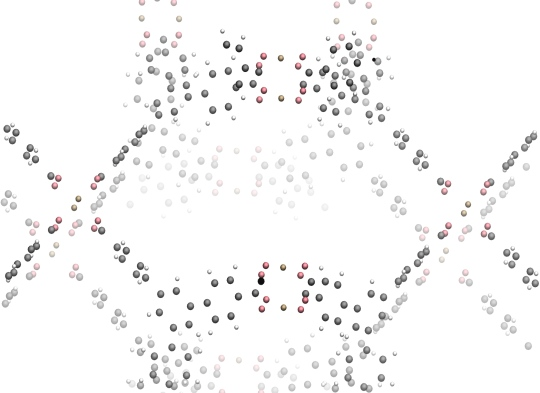
\includegraphics[width=0.95\linewidth]{figures/topology/mof14_0.jpg}
		\caption{Atomes du MOF-143 \autocite{MOF143}}
	\end{subfigure}%
	\begin{subfigure}{0.5\linewidth}
		\centering
		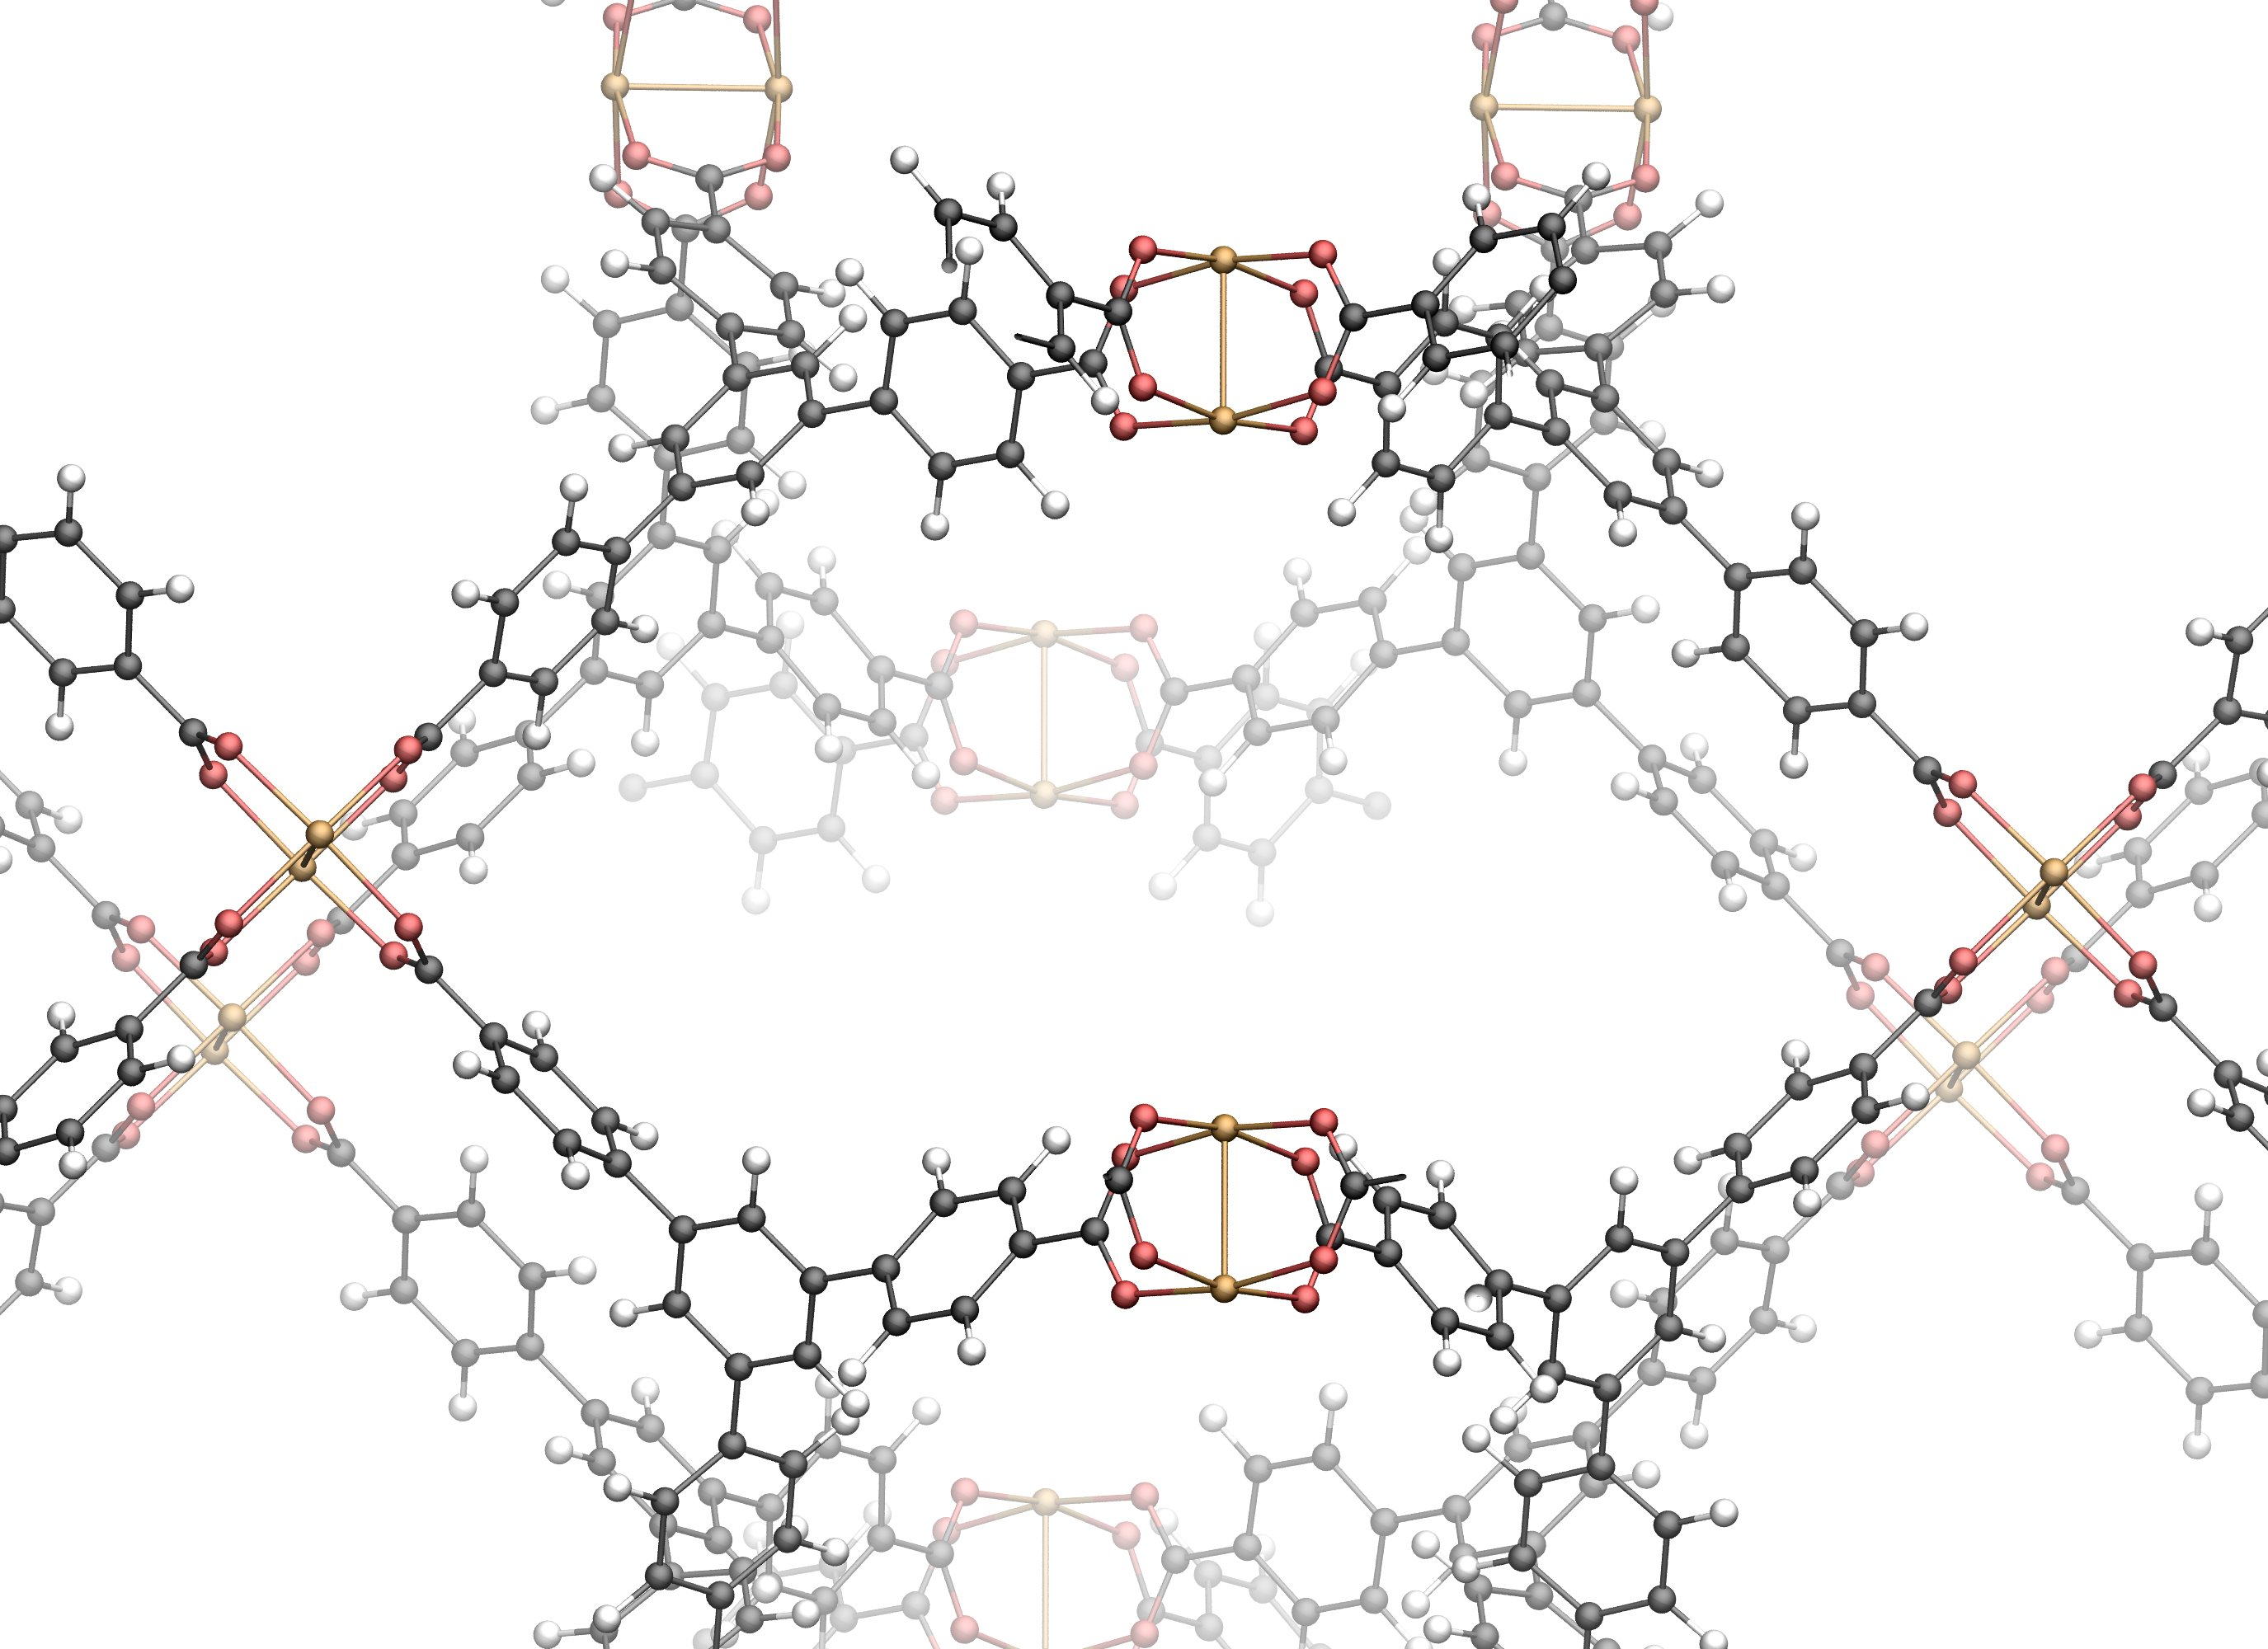
\includegraphics[width=0.95\linewidth]{figures/topology/mof14_1.jpg}
		\caption{Détection des liaisons}
	\end{subfigure}

\vspace{1em}

	\begin{subfigure}{0.5\linewidth}
		\centering
		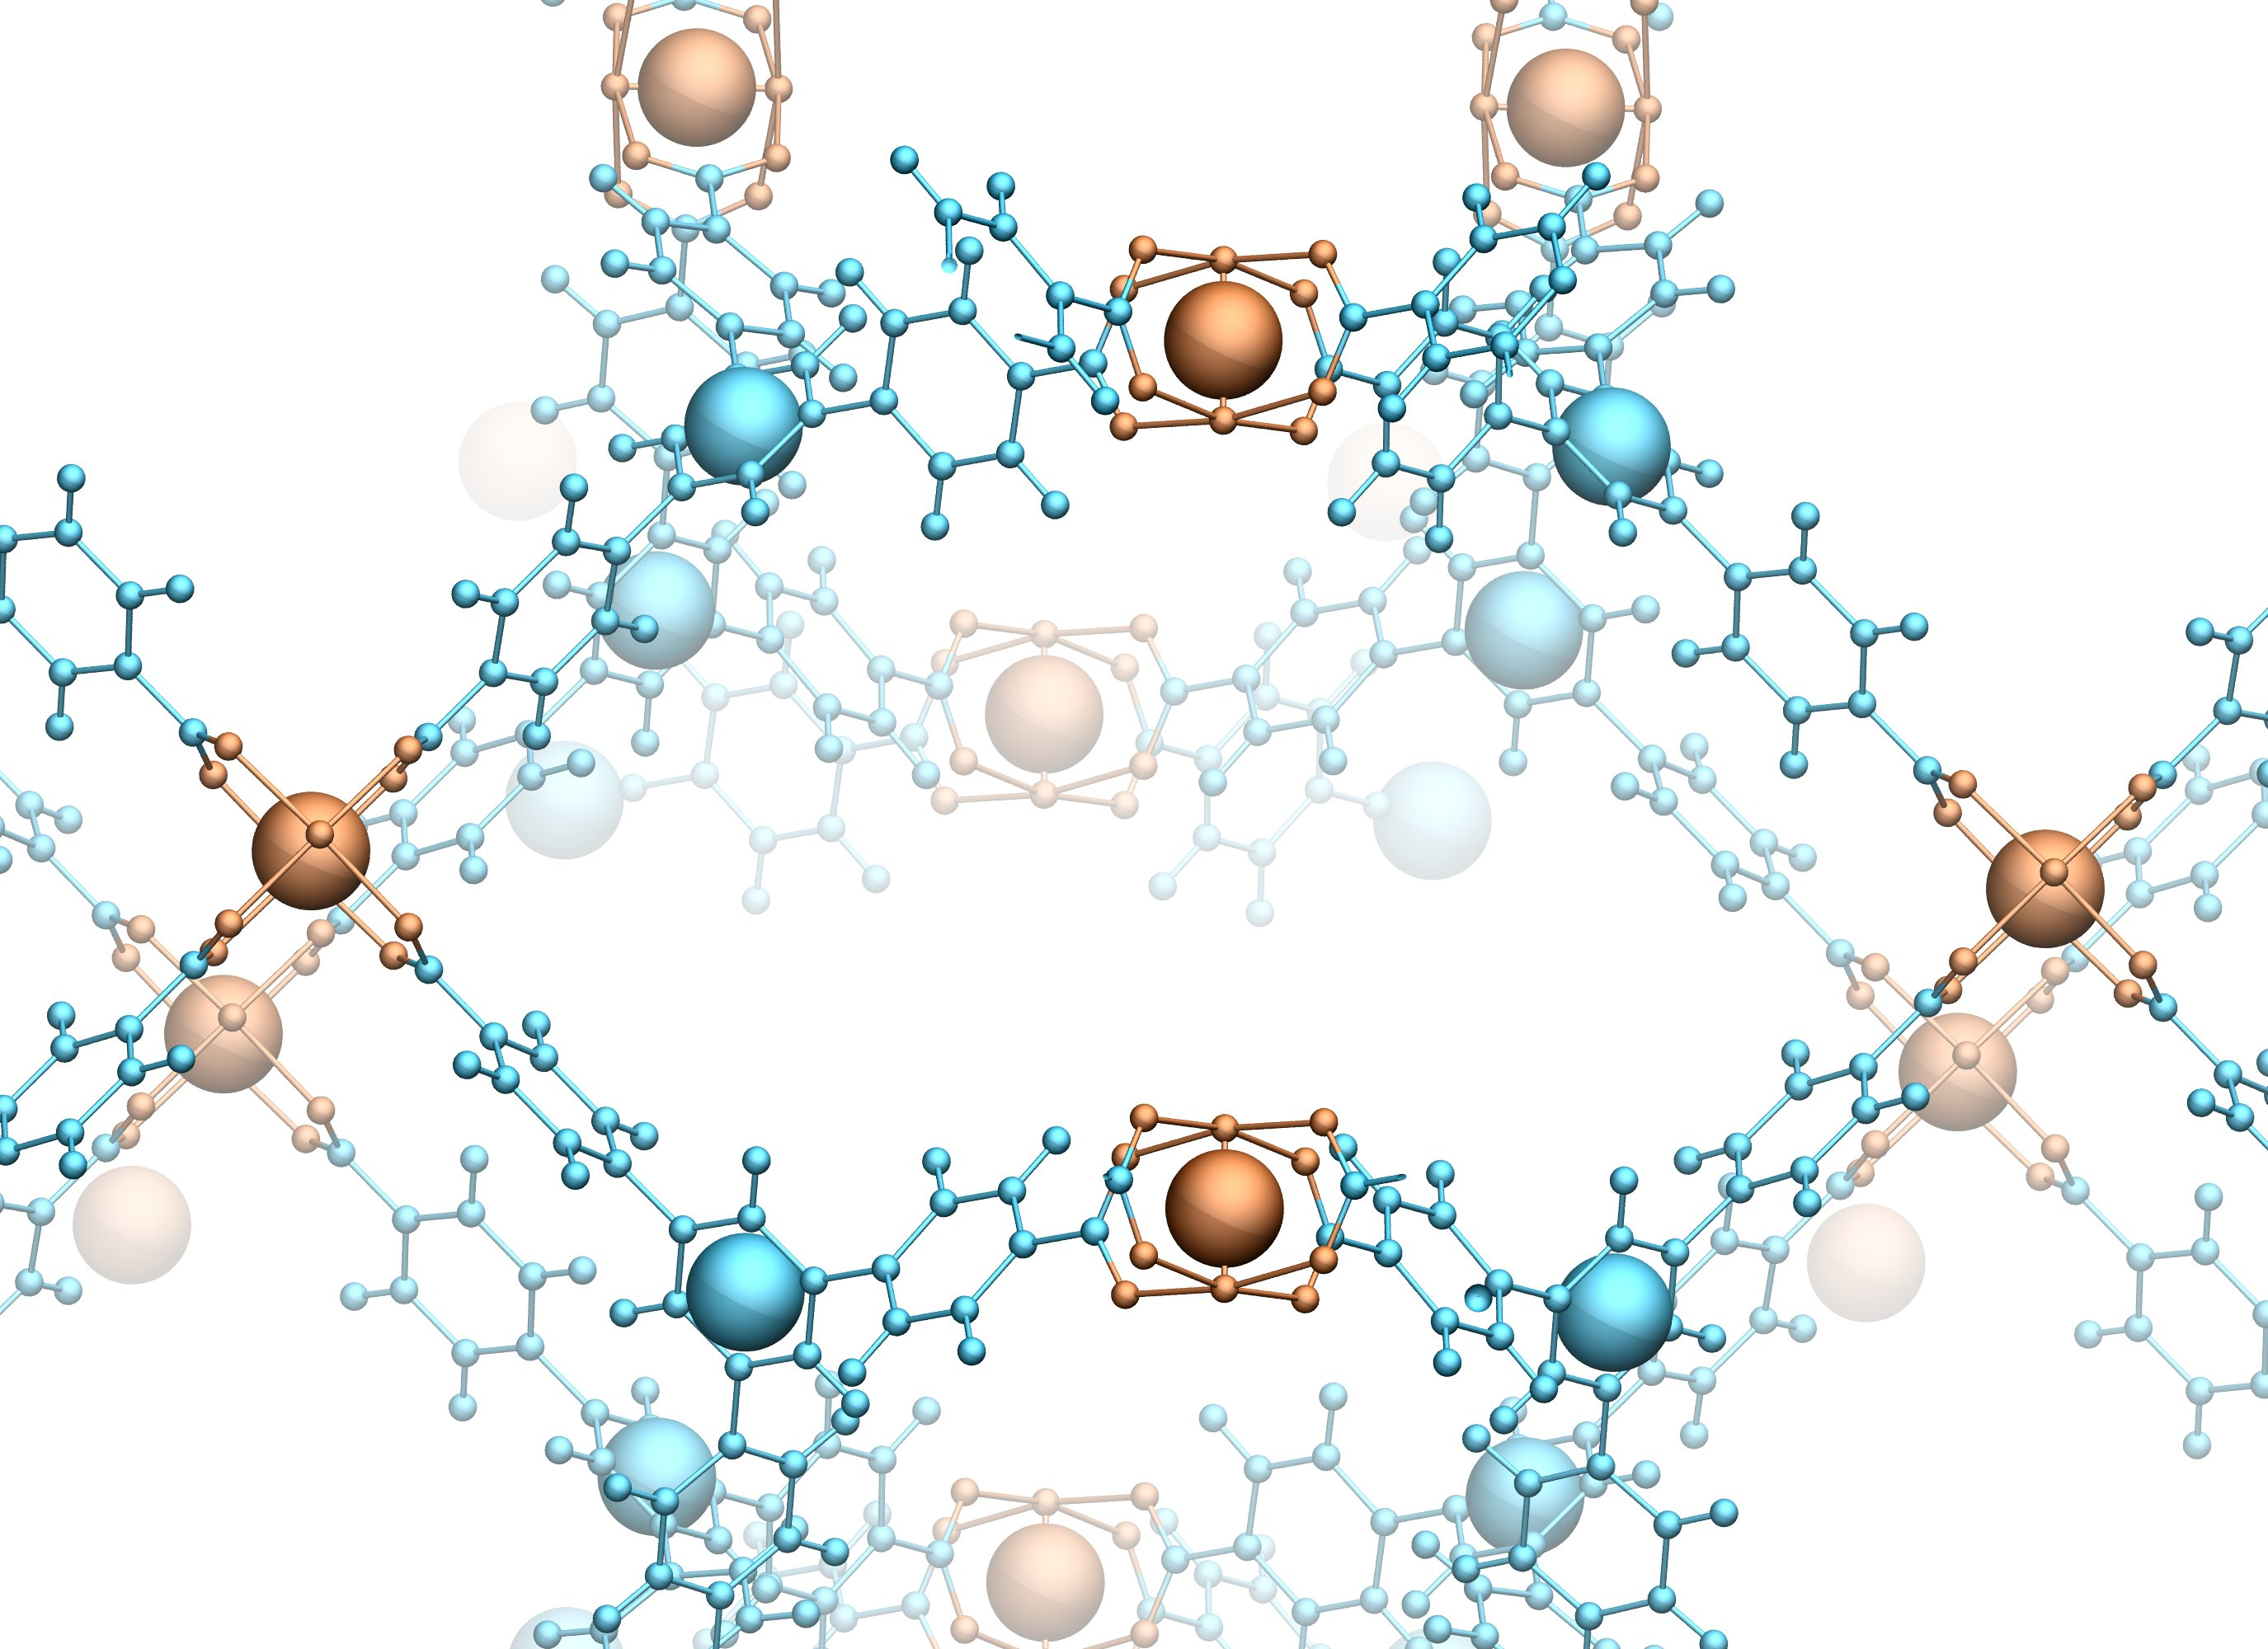
\includegraphics[width=0.95\linewidth]{figures/topology/mof14_2.jpg}
		\caption{Regroupement des atomes en n\oe uds}
	\end{subfigure}%
	\begin{subfigure}{0.5\linewidth}
		\centering
		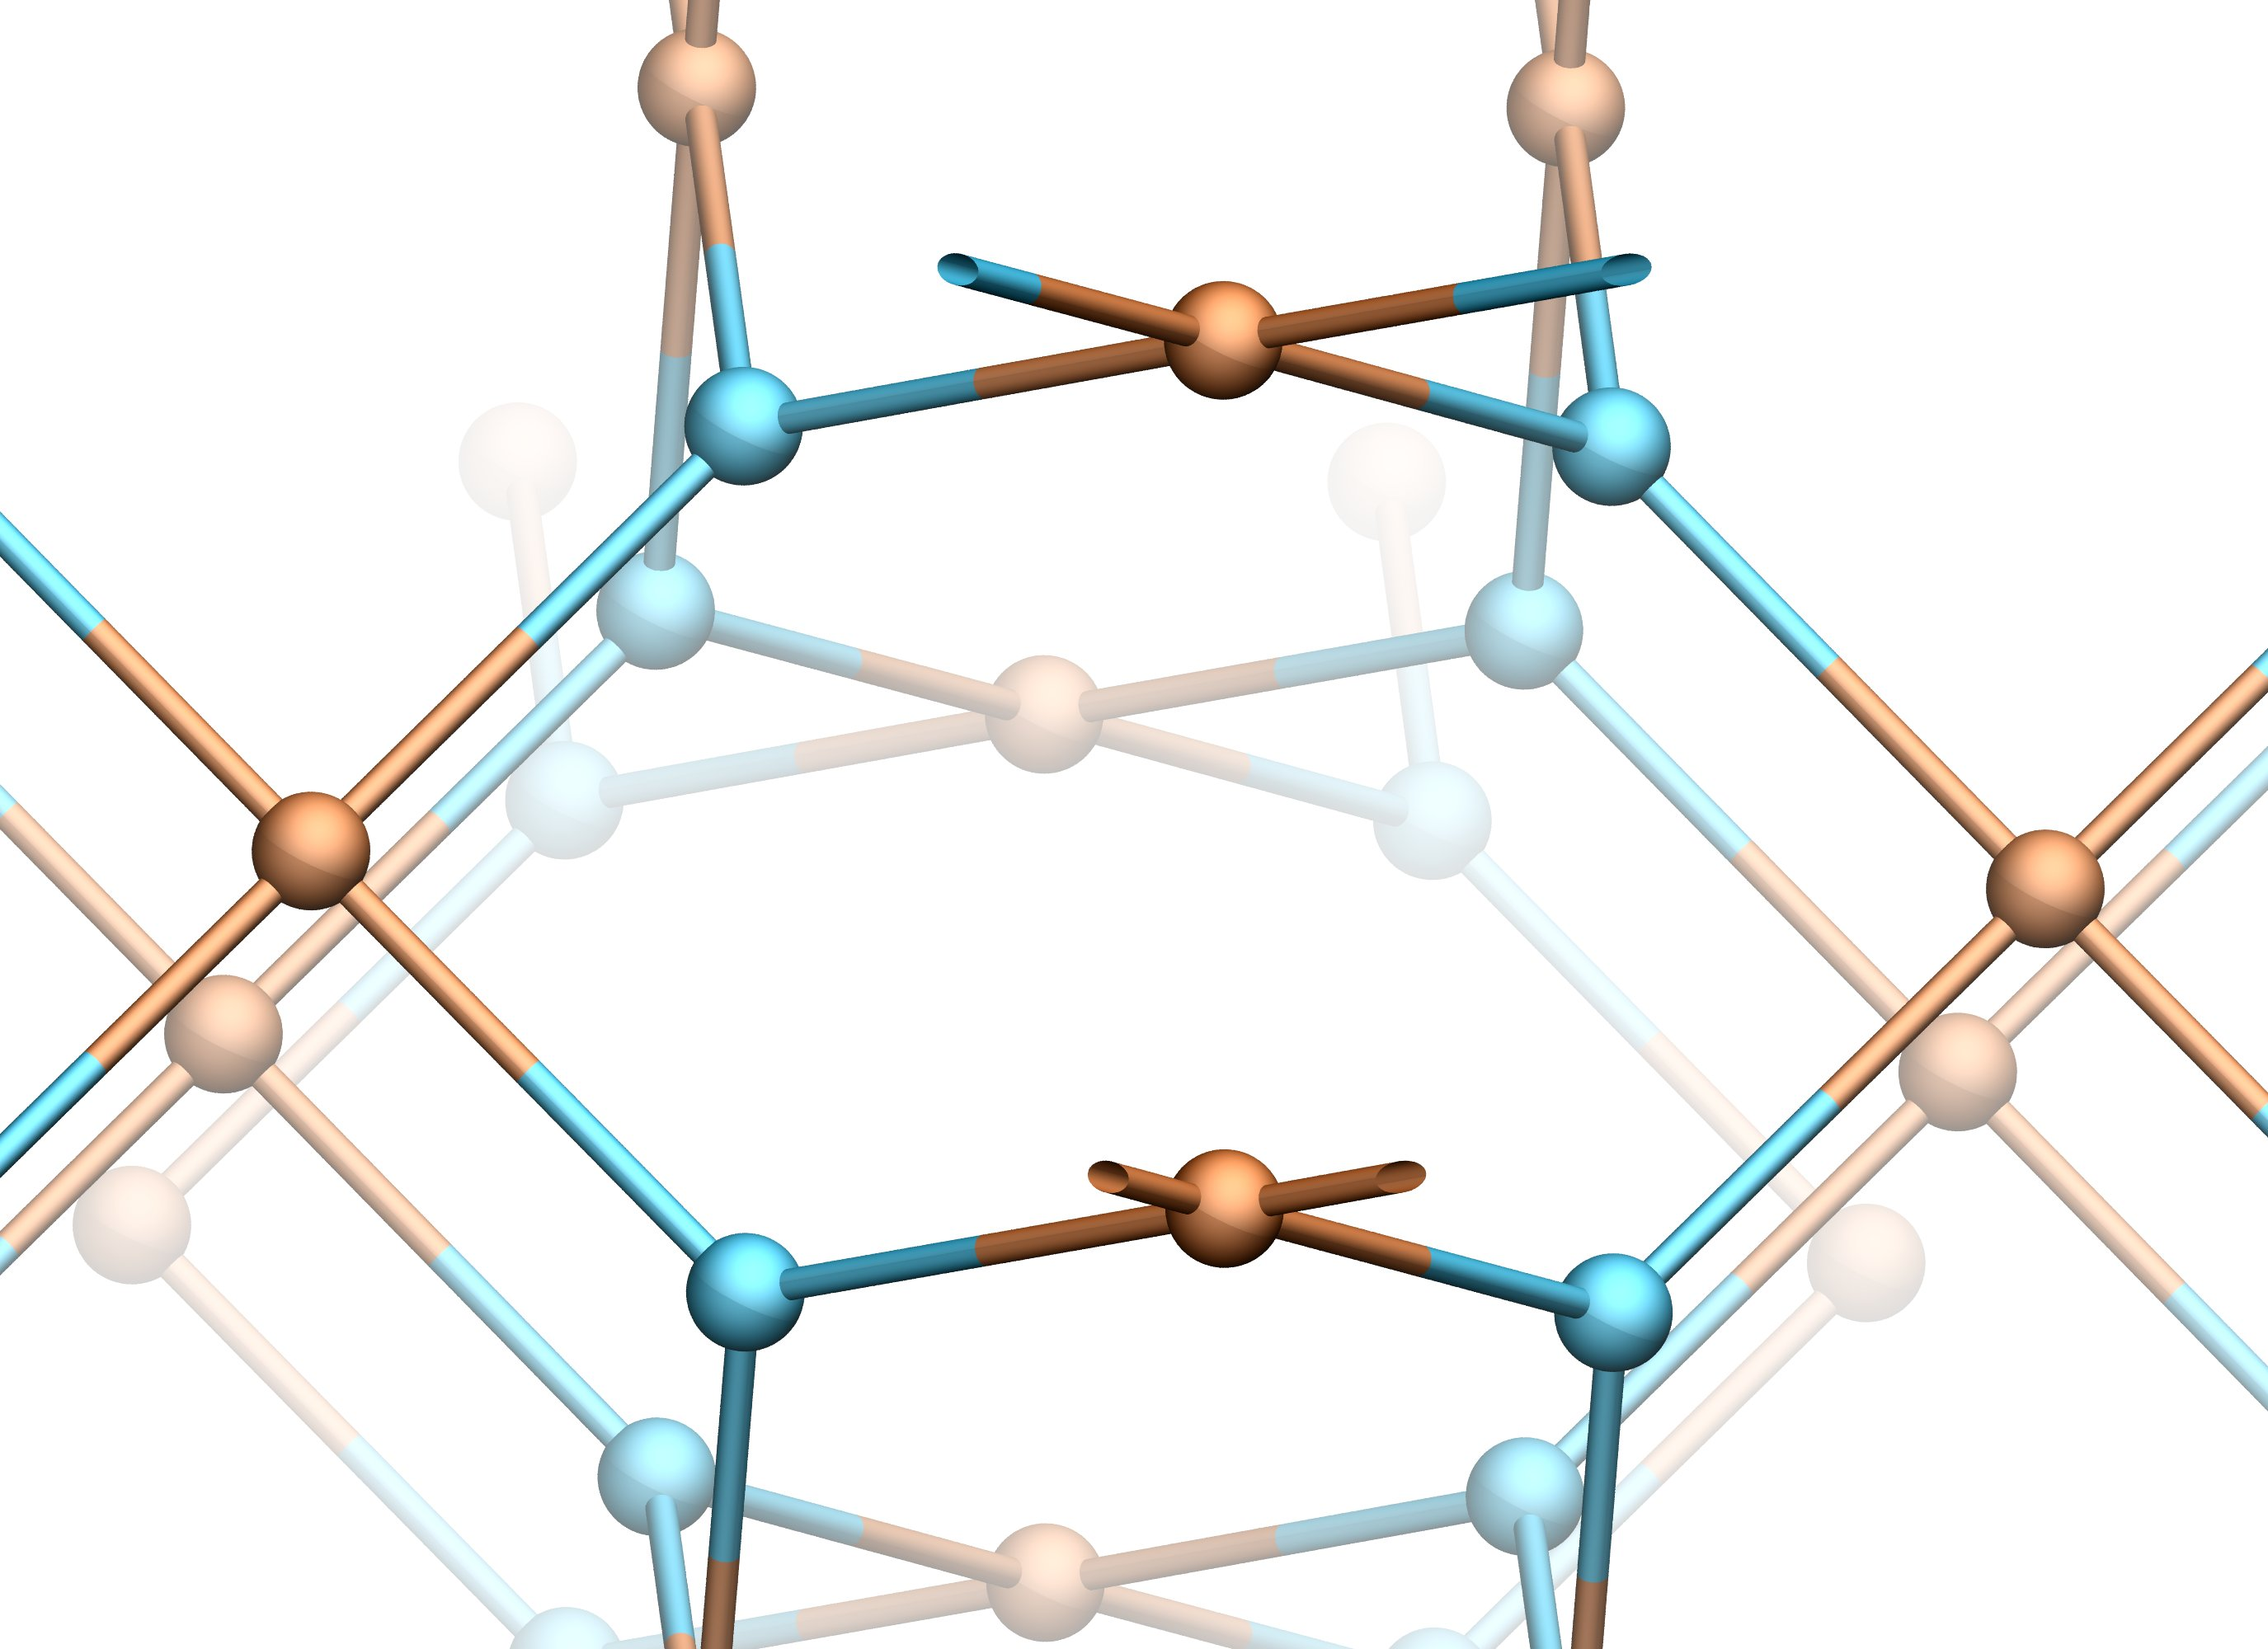
\includegraphics[width=0.95\linewidth]{figures/topology/mof14_3.jpg}
		\caption{Filet sous-jacent (\textbf{pto} dans le RCSR)}
	\end{subfigure}

	\caption{Décomposition d'un MOF en son filet sous-jacent}\label{fig_decompositionfilet}
\end{figure}

La chimie réticulaire \autocite{reticularChemistry,reticularSynthesis} propose de classifier les matériaux en fonction de leur topologie. Cela consiste à simplifier leur structure atomique en regroupant ensemble les atomes partageant la même fonction chimique -- par exemple les noyaux métalliques des réseaux organo-métalliques (\textit{metal-organic frameworks} en anglais, MOF)-- en des ``n\oe uds''. Les liaisons chimiques lient ensuite ces n\oe uds entre eux par des ``arêtes'', de sorte que le réseau des liaisons chimiques est simplement représenté par un graphe, appelé ``filet''. Pour un matériau cristallin, ce filet est périodique, tout comme la structure atomique qu'il sous-tend. Cette décomposition est illustrée par la \cref{fig_decompositionfilet}.

Plusieurs projets recensent les filets correspondant à des cristaux obtenus expérimentalement ou théoriquement. Le RCSR \autocite{RCSR} en particulier contient la description de la plupart des filets communs ; EPINET \autocite{EPINET} contient une liste de très nombreux filets obtenus théoriquement ; enfin, l'Association Internationale des Zéolites \autocite{IZA} liste la totalité des topologies de zéolites connues. La connaissance de la topologie d'un matériau permet ainsi de le comparer à d'autres structures semblables.

Cependant, déterminer le nom de la topologie à partir de la description atomique d'un matériau cristallin est une opération délicate. Historiquement, ceci était réalisé par un expert qui devait reconnaître la topologie à vue, mais cette méthode n'est pas fiable, et difficile d'accès. Depuis, deux outils informatiques ont été développés pour permettre une reconnaissance automatique : ToposPro \autocite{ToposPro,TopCryst} et Systre \autocite{Systre}. ToposPro est un logiciel propriétaire qui fonctionne sous Windows et permet un contrôle fin sur la définition des n\oe uds du filet à utiliser. En contrepartie, il est assez difficile à prendre en main, et son algorithme de reconnaissance des topologies est approximatif, même s'il fonctionne très bien en pratique. Une interface web, TopCryst \autocite{TopCryst}, permet d'identifier gratuitement la topologie d'un matériau, mais n'est pas très performante pour les grosses structures. Systre est un utilitaire open-source qui fonctionne sur n'importe quelle plateforme et qui utilise un algorithme exact pour identifier les matériaux poreux. En revanche, ce logiciel n'accepte en entrée que le filet lui-même, sous un format spécifié, et non pas la description atomistique du matériau, ce qui le rend difficile d'accès.

J'ai développé durant ma thèse le logiciel \texttt{CrystalNets.jl}, écrit en Julia, qui permet d'identifier efficacement la topologie des matériaux cristallins. Celui-ci est open source, accepte de nombreux formats de fichier cristallographique en entrée, et utilise un algorithme exact inspiré de celui de Systre tout en ayant une performance largement supérieure. Son interface web permet d'utiliser très facilement le logiciel sans avoir à programmer, tout en gardant de nombreuses options disponibles, et d'un panneau de visualisation qui garantit que la topologie identifiée correspond bien au cristal donné.

\subsection{Algorithme de \texttt{CrystalNets.jl}}

En partant de la nature et la position des atomes dans une maille du matériau étudié, l'objectif de \texttt{CrystalNets.jl} est d'obtenir le nom de la topologie sous-jacente. Ce travail se décompose en plusieurs parties. Tout d'abord, le réseau des liaisons chimiques est identifié. Puis, les atomes sont regroupés en n\oe uds, de façon à obtenir le filet. Enfin, un ``génome topologique'' est calculé sur le filet : ce génome est une série de nombres, unique pour chaque filet, et qui ne dépend que du filet et pas de sa représentation. Le génome est ensuite comparé à des tables de génomes pré-calculées sur les bases de données du RCSR, EPINET et des zéolites : s'il correspond à une de ces valeurs, le nom correspondant est celui de la topologie.

\subsubsection{Identification des liaisons}

Pour la première étape, la difficulté principale est que la notion de liaison chimique n'est pas définie mathématiquement, elle dépend d'une convention. À défaut d'être parfaite, la stratégie que j'utilise consiste à déterminer si deux atomes sont liés en fonction de leur distance et de leurs rayons de van der Waals. Un certain nombre d'heuristiques sont ensuite employées pour corriger le résultat et obtenir des liaisons plus réalistes : par exemple, la valence des éléments des premières périodes sont limitées. Une stratégie particulière est utilisée pour les liaisons hydrogène, qui dépend de la distance mais aussi de l'angle de la liaison.

\subsubsection{Regroupement en n\oe uds}

Une fois les liaisons établies, des groupes d'atomes sont formés. Plusieurs conventions existent pour effectuer cette tâche : les deux recommandées par l'IUPAC sont ``Single Node'', consistant à prendre un n\oe ud par groupes d'atomes métalliques et un n\oe ud par groupe d'atomes organiques, et ``All Nodes'', avec les mêmes n\oe uds inorganiques mais d'autres n\oe uds organiques, un par point de jonction entre un groupe organique et un groupe métallique dans le regroupement précédent. J'ai implémenté ces deux stratégies, ainsi que quelques autres présentes dans la littérature.

Les n\oe uds sont ensuite liés de sorte à préserver les liaisons chimiques : si deux atomes étaient liés, alors soit ils sont dans le même n\oe ud, soit leurs deux n\oe uds sont liés. Un n\oe ud n'ayant qu'un ou aucun voisin est supprimé, et si un n\oe ud a deux voisins, il est transformé en arêtes entre ceux-ci ; et ce, itérativement jusqu'à convergence.

\subsubsection{Génome topologique}

\begin{figure*}[t]
	\begin{subfigure}[b]{0.35\linewidth}
		\hspace{-1.5em}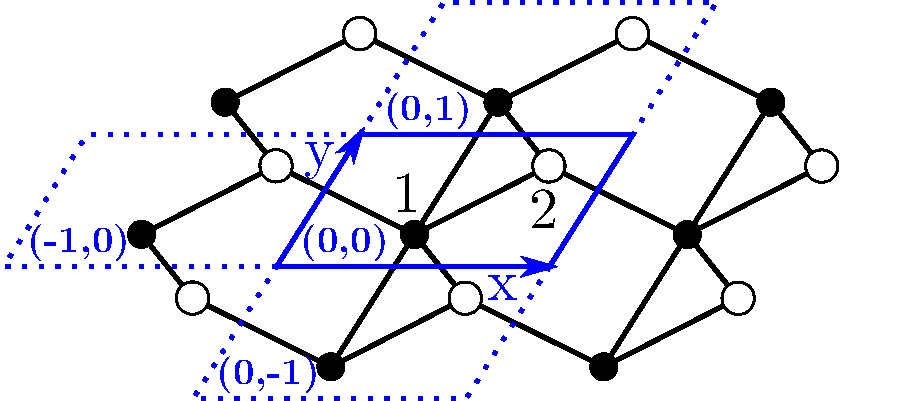
\includegraphics[width=0.96\linewidth]{figures/topology/cells_ref.pdf}
		\subcaption{Maille élémentaire de référence}
		
		\centering\begin{tabular}{ccccc}
			1&1&&0&1\\
			1&2&&-1&0\\
			1&2&&0&-1\\
			1&2&&0&0
		\end{tabular}
		
	\end{subfigure}%
	\begin{subfigure}[b]{0.35\linewidth}
		\hspace{-1.5em}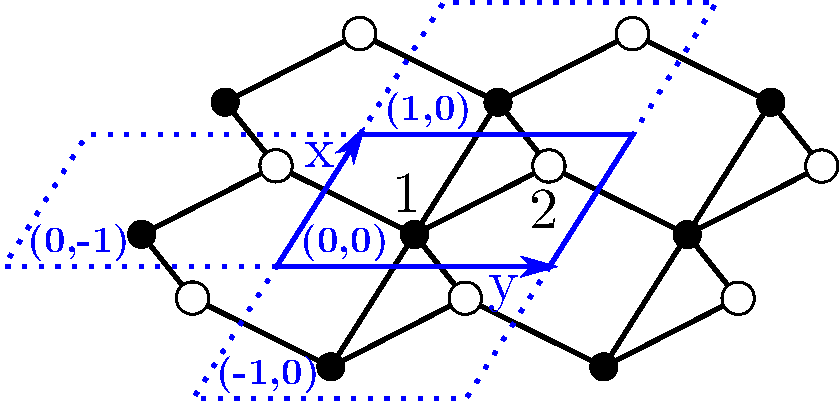
\includegraphics[width=0.9\linewidth]{figures/topology/cells_xy.pdf}
		\subcaption{Inversion des axes}
		
		\centering\begin{tabular}{ccccc}
			1&1&&1&0\\
			1&2&&-1&0\\
			1&2&&0&-1\\
			1&2&&0&0
		\end{tabular}
		
	\end{subfigure}%
	\begin{subfigure}[b]{0.35\linewidth}
		\hspace{-2em}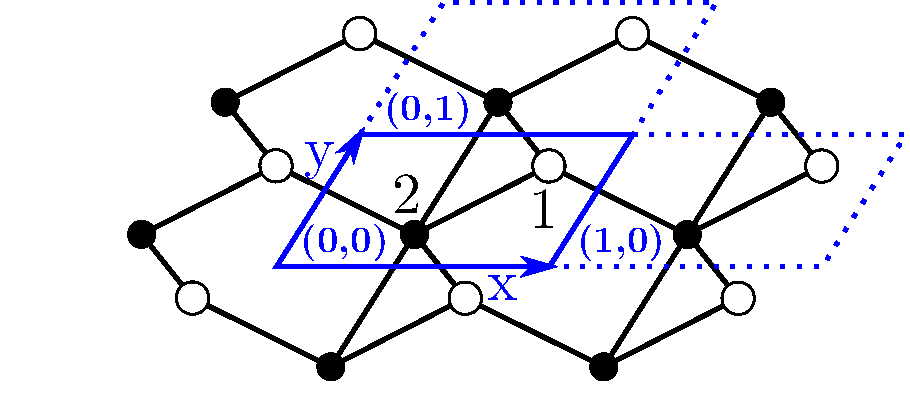
\includegraphics[width=1\linewidth]{figures/topology/cells_12.pdf}
		\subcaption{Numérotation des n\oe uds}
		
		\centering\begin{tabular}{ccccc}
			1&2&&0&0\\
			1&2&&0&1\\
			1&2&&1&0\\
			2&2&&0&1
		\end{tabular}
		
	\end{subfigure}
	\begin{subfigure}[b]{0.35\linewidth}
		\hspace{1.5em}
		\hspace{-2em}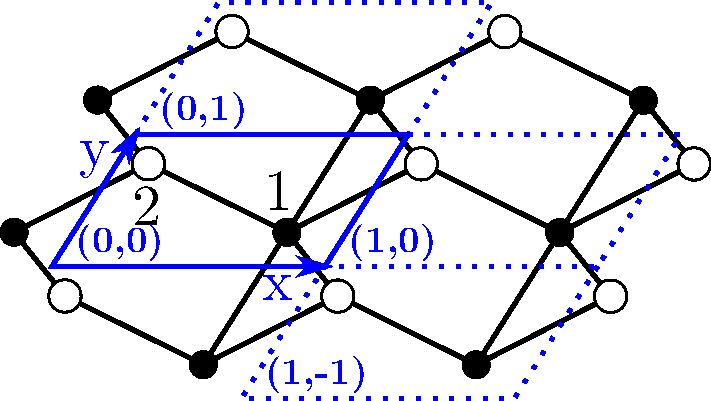
\includegraphics[width=0.8\linewidth]{figures/topology/cells_orig.pdf}
		\vspace{1em}
		\subcaption{Changement d'origine}
		
		\centering\begin{tabular}{ccccc}
			1&1&&0&1\\
			1&2&&0&0\\
			1&2&&1&-1\\
			1&2&&1&0
		\end{tabular}
		\vspace{-0.5em}
	\end{subfigure}%
	\begin{subfigure}[b]{0.35\linewidth}
		\hspace{-2em}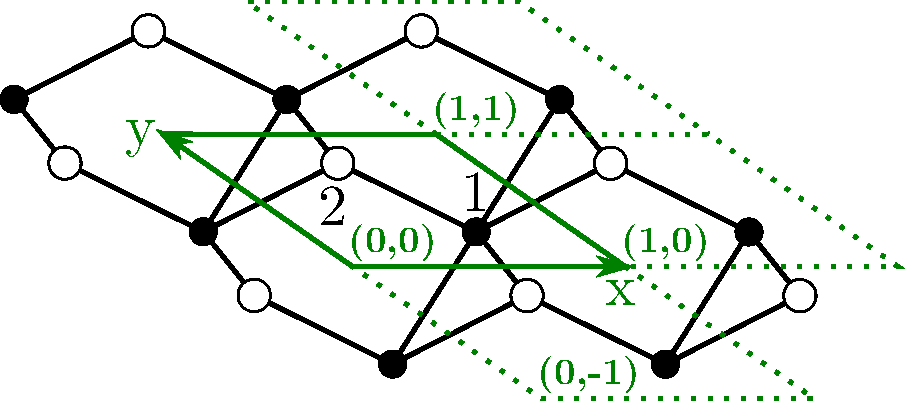
\includegraphics[width=1\linewidth]{figures/topology/cells_other.pdf}
		\vspace{1em}
		\subcaption{Autre maille élémentaire}
		
		\centering\begin{tabular}{ccccc}
			1&1&&1&1\\
			1&2&&0&-1\\
			1&2&&0&0\\
			1&2&&1&0
		\end{tabular}
		\vspace{-0.5em}
	\end{subfigure}%
	\begin{subfigure}[b]{0.35\linewidth}
		\centering
		\hspace{-2em}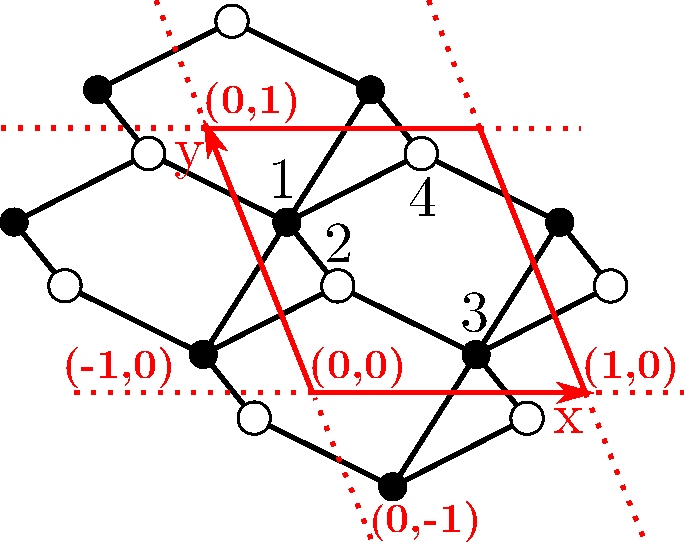
\includegraphics[width=0.63\linewidth]{figures/topology/cells_super.pdf}
		\vspace{-0.5em}
		\subcaption{Maille non-élémentaire}
		
		\centering\scriptsize\begin{tabular}{ccccc}
			1&2&&0&0\\
			1&3&&-1&0\\
			1&3&&0&1\\
			1&4&&-1&0\\
			1&4&&0&0\\
			2&3&&-1&0\\
			2&3&&0&0\\
			3&4&&0&-1
		\end{tabular}
		\vspace{-0.5em}
	\end{subfigure}
	\vspace{2mm}
	\caption{Six représentations différentes du même filet bidimensionnel, avec leur clé. Les deux premières colonnes contiennent les numéros des n\oe uds de départ et d'arrivée, les deux suivantes sont le décalage des maille entre le départ et l'arrivée.} \label{fig_cles}
\end{figure*}

À ce stade, le matériau a été simplifié en sous filet sous-jacent. Un filet est représenté numériquement comme la liste de ses arêtes, chaque arête étant constituée du numéro du n\oe ud de départ, celui d'arrivée, et la différence entre les décalage des mailles contenant chacun des deux n\oe uds, qui s'exprime comme autant d'entiers que de dimension du filet. Pour un matériau tridimensionnel, chaque arête est donc représentée par cinq entiers ; en triant les arêtes lexicographiquement on obtient ainsi une ``clé'', qui est une série de nombre.

Une clé correspond toujours au même filet, en revanche un filet peut être représenté par différentes clé, selon le choix de la maille élémentaire ou de la numérotation des n\oe uds, comme représenté sur la \cref{fig_cles}. Pour trouver le génome topologique, qui doit être vraiment unique, Systre prend la plus petite clé parmi un ensemble calculé de façon à être indépendant de la représentation de départ du filet. \texttt{CrystalNets.jl} procède de même, mais utilise un ensemble plus réduit de clés, et les calcule plus efficacement, ce qui garantit la sûreté de l'algorithme tout en offrant une meilleure performance.

\subsection{Analyse de bases de données de structures}

La vitesse de \texttt{CrystalNets.jl} lui permet d'être employé dans le cadre de criblage de matériaux à haut débit. J'ai ainsi pu analyser plusieurs bases de données de structures et obtenir les distributions de topologies associées.

Parmi celles-ci, la base de données CoRE-MOF 2019 \autocite{CoREMOF2024} est très utilisée pour l'analyse numérique des MOFs. Deux topologies sont particulièrement surreprésentées : \textbf{pcu}, la topologie la plus simple où chaque n\oe ud est connecté à ses voisins comme une grille régulière tridimensionnelle, et \textbf{dia}, la topologie des carbones dans le diamant.

J'ai aussi utilisé \texttt{CrystalNets.jl} pour analyser les topologies de la base de donnée CoRE-MOF 2024 actuellement en cours d'élaboration. Les deux topologies précédentes restent en tête, mais sont immédiatement suivies de \textbf{sql}, l'équivalent bidimensionnel de \textbf{pcu}. Ceci indique un enrichissement de la base de données, puisque de nouvelles topologies ne peuvent correspondre qu'à de nouvelles structures.

\subsection{Interface web CrystalNets}

Pour rendre le logiciel plus facilement accessible, en particulier aux expérimentateurs qui souhaitent pouvoir facilement accéder à l'analyse topologique de leur matériau sans nécessairement devoir programmer, j'ai construit une interface web accessible à l'adresse suivante : \url{https://progs.coudert.name/topology}, représentée sur la \cref{fig_webcrystalnets}.

\begin{figure}[b]`
	\centering
	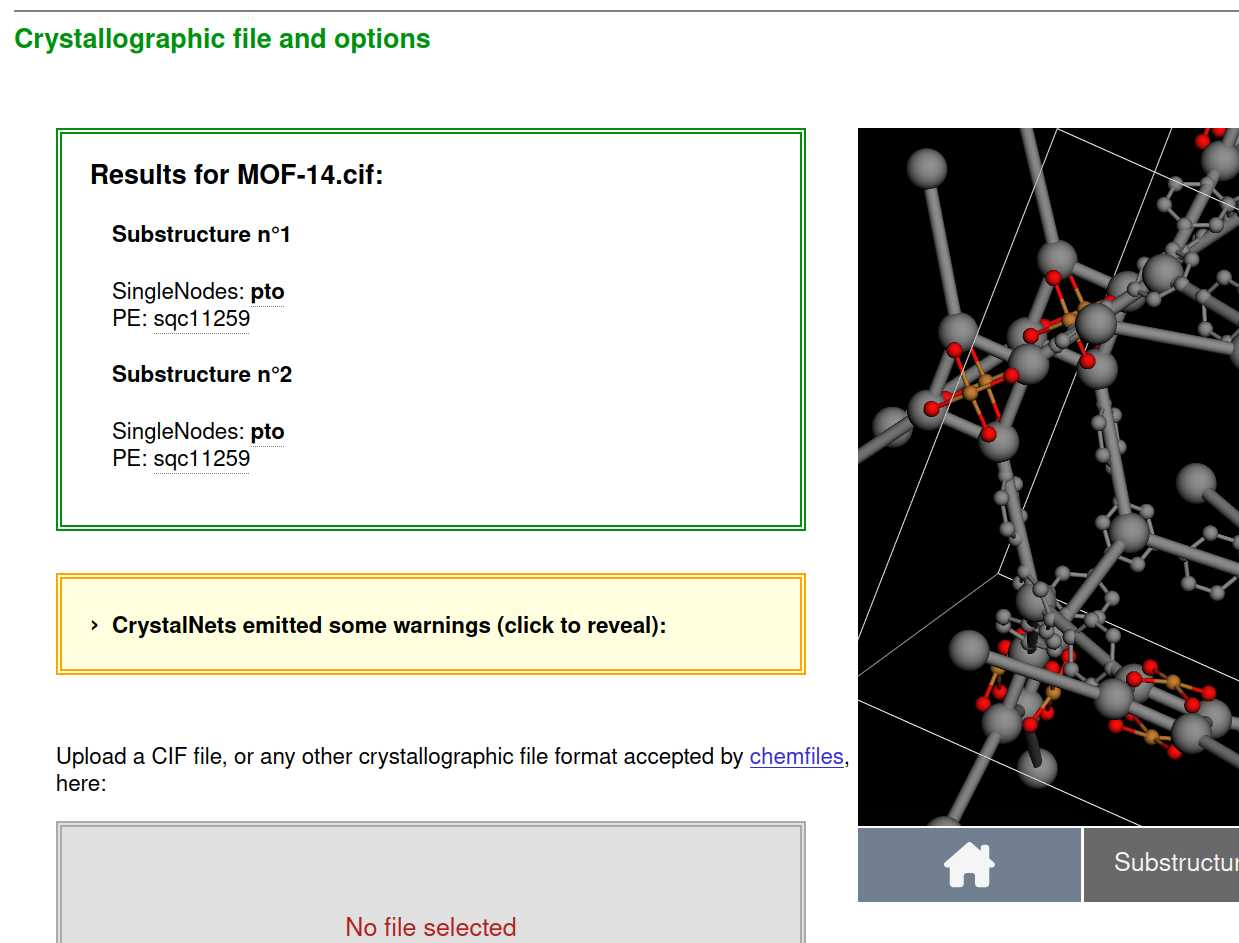
\includegraphics[width=0.9\linewidth]{figures/topology/WebsiteAnswer.jpg}
	\caption{Capture d'écran du résultat d'une analyse topologique réalisée sur l'interface web CrystalNets. Dans l'encadré vert : la topologie pour chaque sous-structure, selon différentes stratégies de regroupement d'atomes. À droite, le panneau de visualisation (tronqué) où le filet est superposé à l'entrée. En bas, l'invite (tronquée) pour déposer une nouvelle structure et relancer une analyse}\label{fig_webcrystalnets}
\end{figure}

La prise en main est très intuitive : il suffit de glisser le fichier cristallographique représentant le matériau étudié dans l'invite, et de choisir les options de détection de liaison et regroupement des atomes, celles-ci possédant des valeurs par défaut généralistes. La structure et ses options sont alors envoyées sur un serveur qui exécute le programme écrit en Julia. Grâce à sa performance optimisée, l'exécution se déroule en quelques secondes au plus dans la très grande majorité des cas. Le serveur renvoie ensuite la topologie identifiée, et présente dans un panneau dédié la superposition de la structure donnée en entrée avec le filet qui a été déterminé.

Cette visualisation est une importante plus-value car elle permet de s'assurer de la qualité de l'analyse du logiciel. Tout particulièrement dans le cas où les liaisons chimiques doivent être identifiées automatiquement, cette vérification est indispensable.


\section{Structure des zéolites cationiques}

\subsection{Généralités}

Les zéolites sont les aluminophosphates cristallins nanoporeux. Cette famille de matériaux est donc structurellement organisée autour de tétraèdres \ce{TO4} où l'atome central T est généralement Si, parfois substitué par Al, et est lié à quatre autres atomes T par le biais d'oxygènes pontant. Les zéolites sont classifiées en fonction de leur topologie, qui s'obtient en prenant pour n\oe ud les atomes T, et pour arêtes les ponts T--O--T : il existe à ce jour 256 topologies distinctes de zéolites connues \autocite{IZA}.

\begin{figure}[ht]
	\centering
	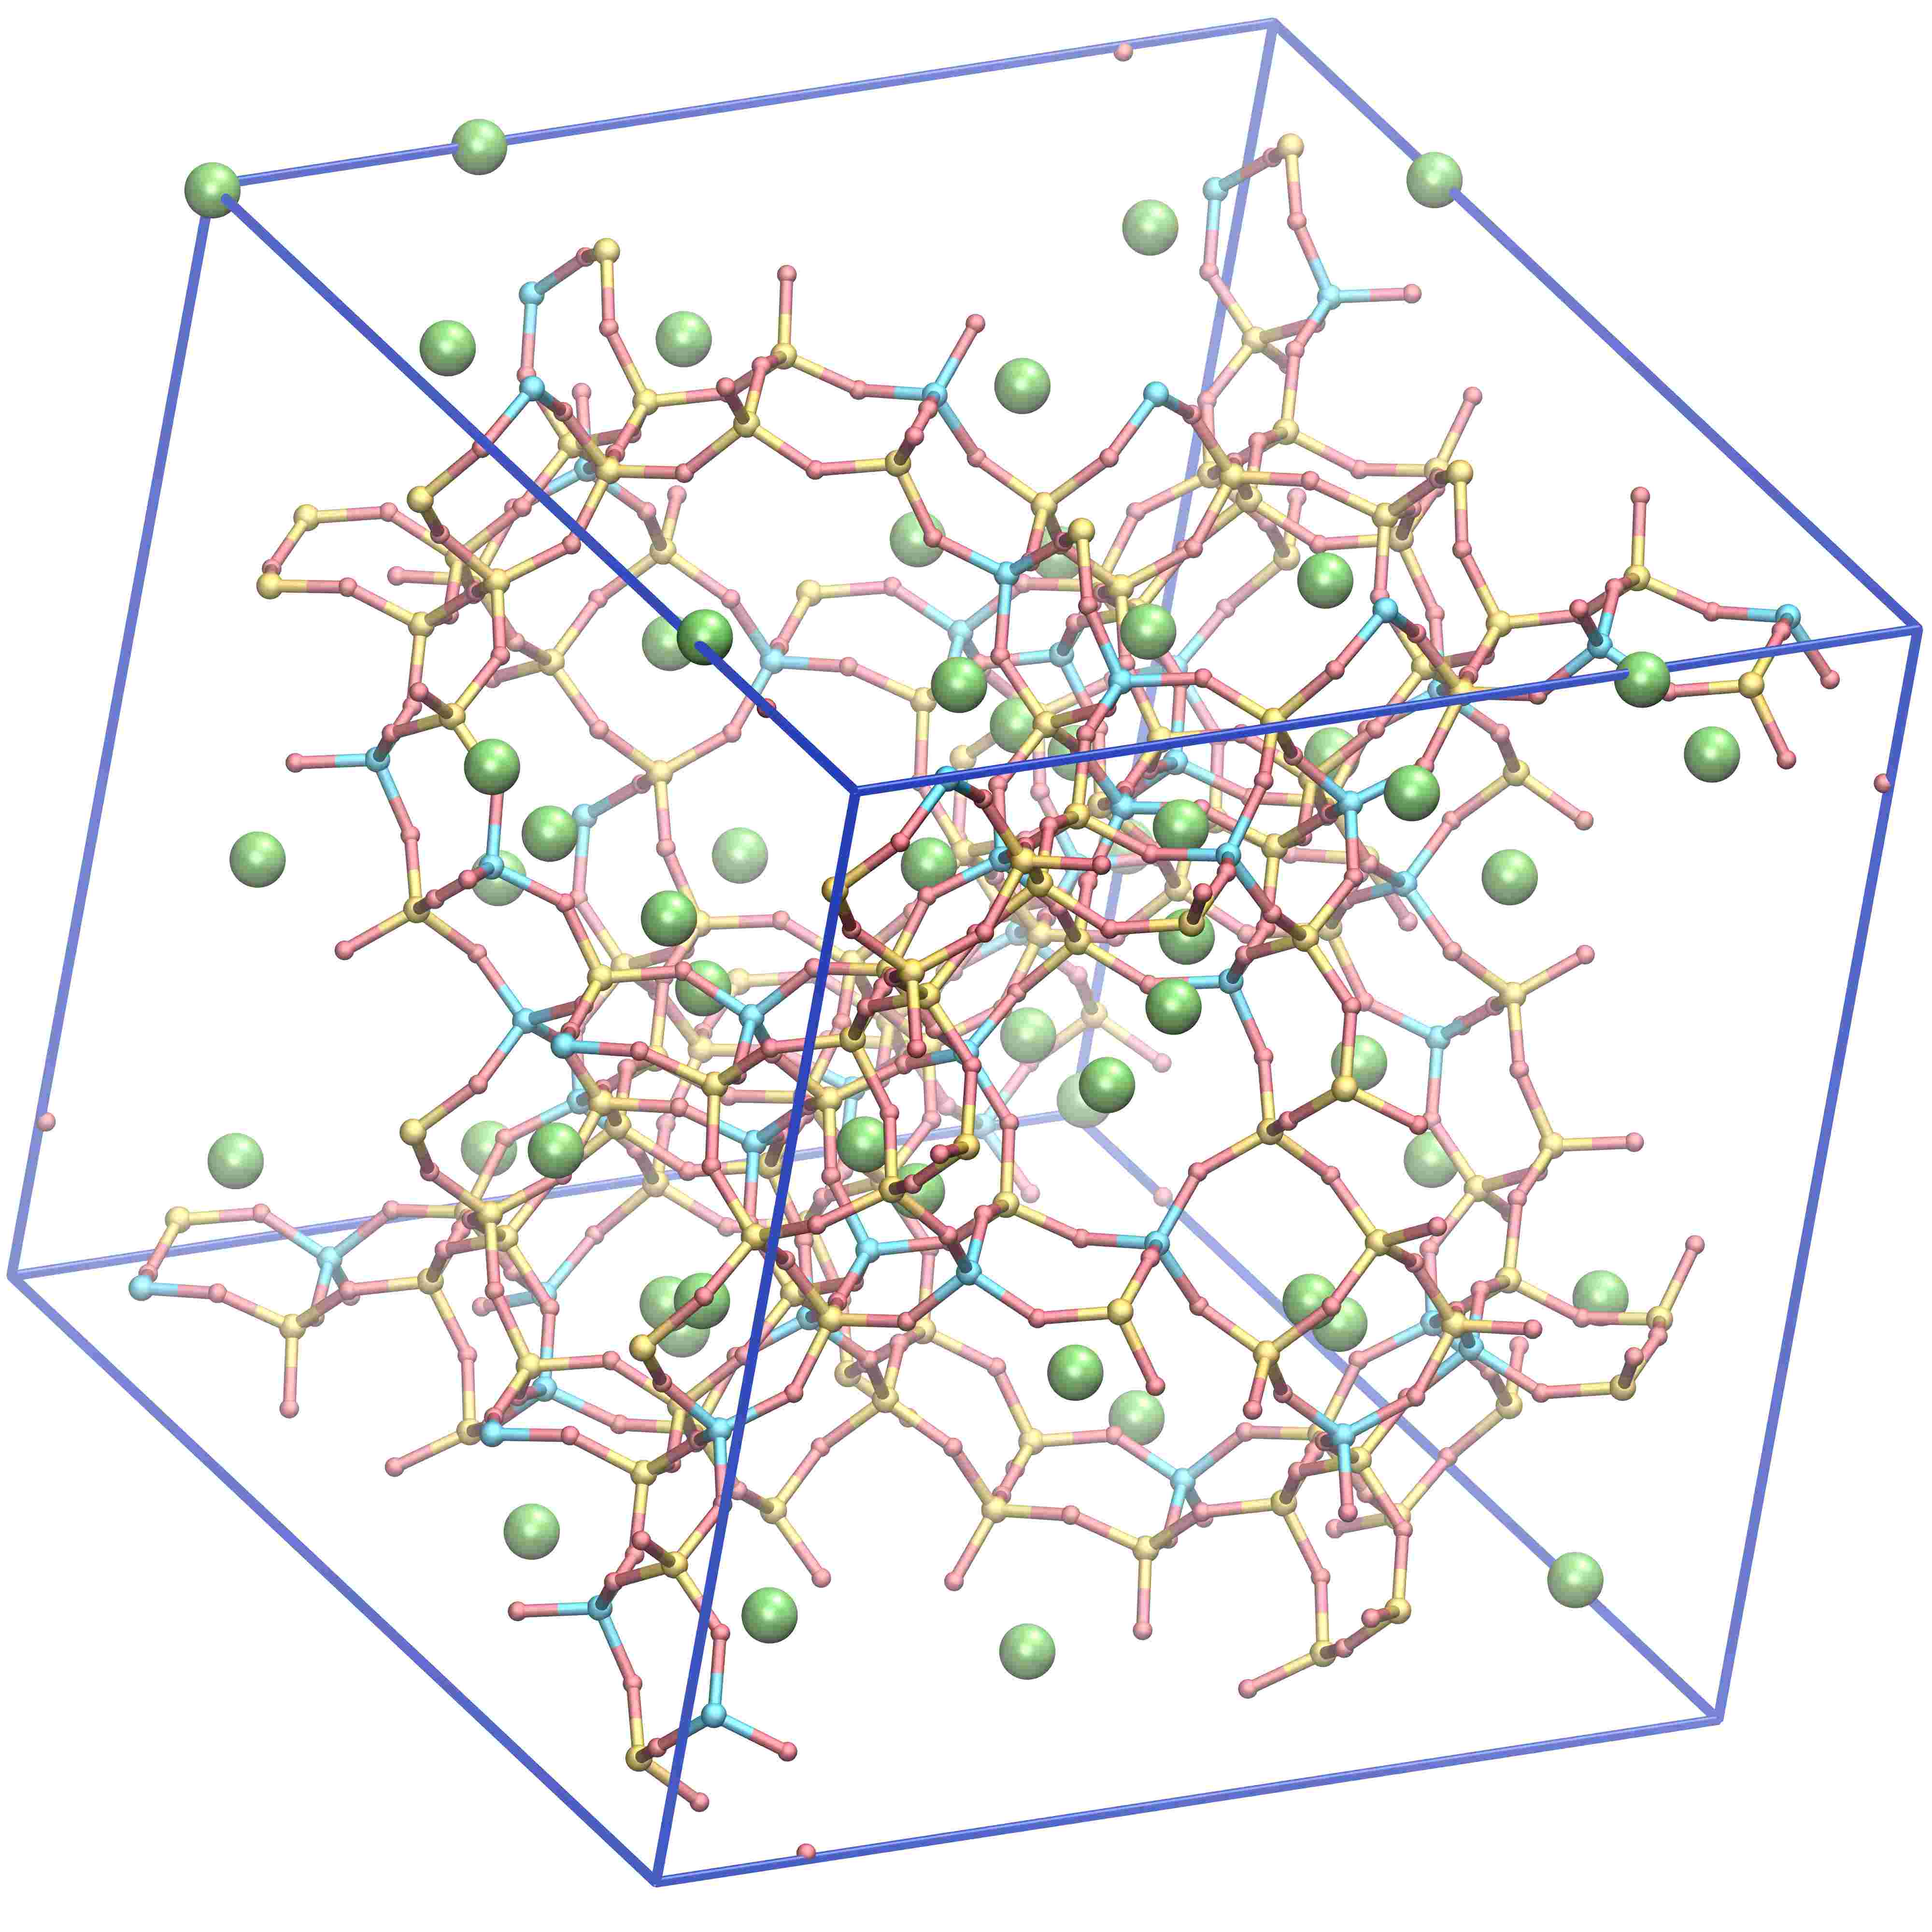
\includegraphics[width=0.8\linewidth]{figures/cations/FAU2.5_framework_Na.jpg}
	\caption{Maille élémentaire d'une zéolite, ici la faujasite. O en rouge, Si en jaune, Al en bleu, ici $\SiAl = 2.5$. Cations extra-charpentes \ce{Na+} en vert.}\label{fig_FAU25}
\end{figure}

Chaque substitution d'un Si par un Al introduit un électron supplémentaire, qui est compensé par la présence de cations. Ceux-ci ne sont pas liés de façon covalente à la charpente, et sont donc libres de circuler. Cependant, les mesures spectrométriques des zéolites indiquent que les cations sont en fait localisés : ils se placent sur certains sites et en bougent très peu. Afin d'obtenir une représentation atomistique raisonnable des zéolites cationiques, il faut donc savoir où sont placés les aluminiums dans la charpentes, et où se localisent les cations extra-charpentes. Une illustration de zéolite est présentée sur la \cref{fig_FAU25}

\subsection{Placement des aluminiums}

Dans le cas des aluminiums, la question n'est pas vraiment élucidée. Il existe en effet peu de moyen expérimental pour déterminer la localisation des aluminiums ; il n'est de plus pas sûr que leur organisation suive la périodicité du matériau. La seule loi connue est la règle de L\"owenstein \autocite{Loewenstein}, qui dit que deux Al ne sont pas jamais voisins.

La nature même de leur positionnement est sujet à controverse. Celui-ci pourrait en effet être guidé par la thermodynamique, c'est-à-dire que les aluminiums se placeraient de façon à minimiser l'énergie globale du matériau. Mais la structure des zéolites est elle-même métastable, et de plusieurs éléments indiquent que l'organisation des aluminiums dépend des conditions de synthèse : dans ce cas, le placement s'effectuerait sous contrôle cinétique.

Afin de traiter un grand nombre de zéolites de façon réaliste et en l'absence d'élément déterminant la validité de l'un ou l'autre de ces modes de contrôle, j'ai décidé de placer les Al au hasard parmi les atomes T, à condition de vérifier la règle de L\"owenstein, et de sélectionner 6 de ces placements pour chaque topologie et chaque rapport \SiAl étudié. Les propriétés d'une zéolite sont ensuite obtenues en moyennant celles résultant de chacun des 6 modèles.

\subsection{Placement des cations}

Une fois les aluminiums placés, il reste à déterminer la position des cations. Il existe des moyens expérimentaux de l'obtenir, mais l'objectif ici est d'obtenir des modèles pour un grand nombre de zéolites, afin de pouvoir réaliser ensuite un traitement statistique.

\subsubsection{Méta-algorithme ``étoile filante''}

Il faut donc effectuer des simulations moléculaires pour trouver la localisation optimale des cations. Leur nombre, le volume de la maille élémentaire, et la température du matériau étant connus, l'ensemble statistique pertinent est l'ensemble canonique, qui peut-être simulé soit par dynamique moléculaire, soit par Monte-Carlo. J'ai choisi d'implémenter cette dernière option, car les contraintes de trajectoire de la première ralentissent fortement la convergence des simulations.

Dans ce cadre, le problème principal est la nature très vallonnée de la surface d'énergie libre du système constitué des cations. En d'autres termes, la simulation de ce système se retrouve très facilement piégée dans un minimum local d'énergie, qui ne permet pas de retrouver le minimum global correspondant à la vraie répartition des cations.

Pour résoudre ce problème, il existe dans la littérature plusieurs méta-algorithmes, comme le recuit simulé ou le \textit{parallel tempering}, qui s'utilisent en combinaison avec l'algorithme de simulation canonique. Ces méta-algorithmes mélangent la simulation à la température souhaitée avec d'autres simulations à des températures beaucoup plus élevées, et pour lesquelles le système n'est pas bloqué par les barrières d'énergie problématiques.

J'ai développé un nouveau méta-algorithme, appelé ``étoile filante'', représenté sur la \cref{fig_shootingstar}, qui consiste à exécuter une simulation ``chaude'' à très haute température (comme le météore), de laquelle sont lancées régulièrement des simulations ``froides'' à la température d'étude (comme la traînée de l'étoile filante). Chaque simulation froide effectue le même nombre de cycles de pas Monte-Carlo, et la convergence du système peut être évaluée à partir de l'évolution de la valeur moyenne de l'énergie des simulations froides en fonction du cycle.

\begin{figure}
	\centering
	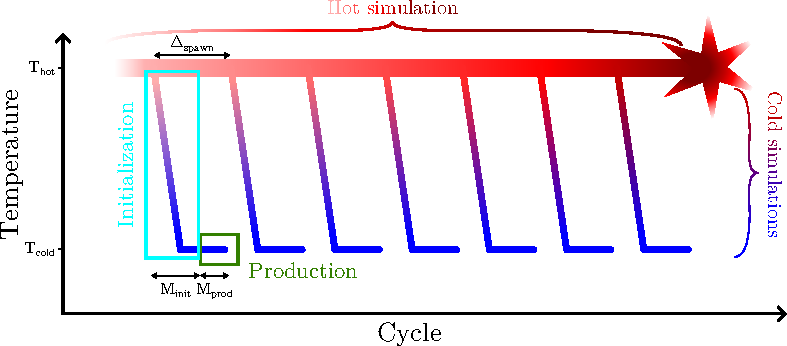
\includegraphics[width=\linewidth]{figures/cations/shootingstar.pdf}
	\caption{Représentation schématique du méta-algorithme ``étoile filante''}\label{fig_shootingstar}
\end{figure}

\subsubsection{Localisation et peuplement des sites cationiques}

Une fois la simulation convergée, les positions prises par les cations au cours de la phase de production de la simulation sont reportées sur une unique carte, qui recense, pour chaque élément de volume pris sur une grille dans la maille, la densité moyenne de cation sur ce volume. Les différents sites cationiques sont ensuite identifiés à partir de cette carte grâce à un algorithme idoine que j'ai développé. Ce procédé est illustré sur la \cref{fig_FAU}.

Une fois les sites identifiés, reste à savoir combien de cations se situe sur chaque site. Pour ce faire, j'ai utilisé une simulation où les cations sont contraints d'être toujours localisé sur un site cationique, et où le seul pas Monte-Carlo autorisé est le saut d'un site vers un autre. Cet algorithme peut lui aussi être augmenté d'un méta-algorithme afin d'accélérer sa convergence : en l'occurrence, le recuit simulé suffit à obtenir un peuplement stable des sites cationiques.

\begin{figure}[ht]
	\centering
	\hfill\begin{subfigure}{0.45\columnwidth}
		\centering
		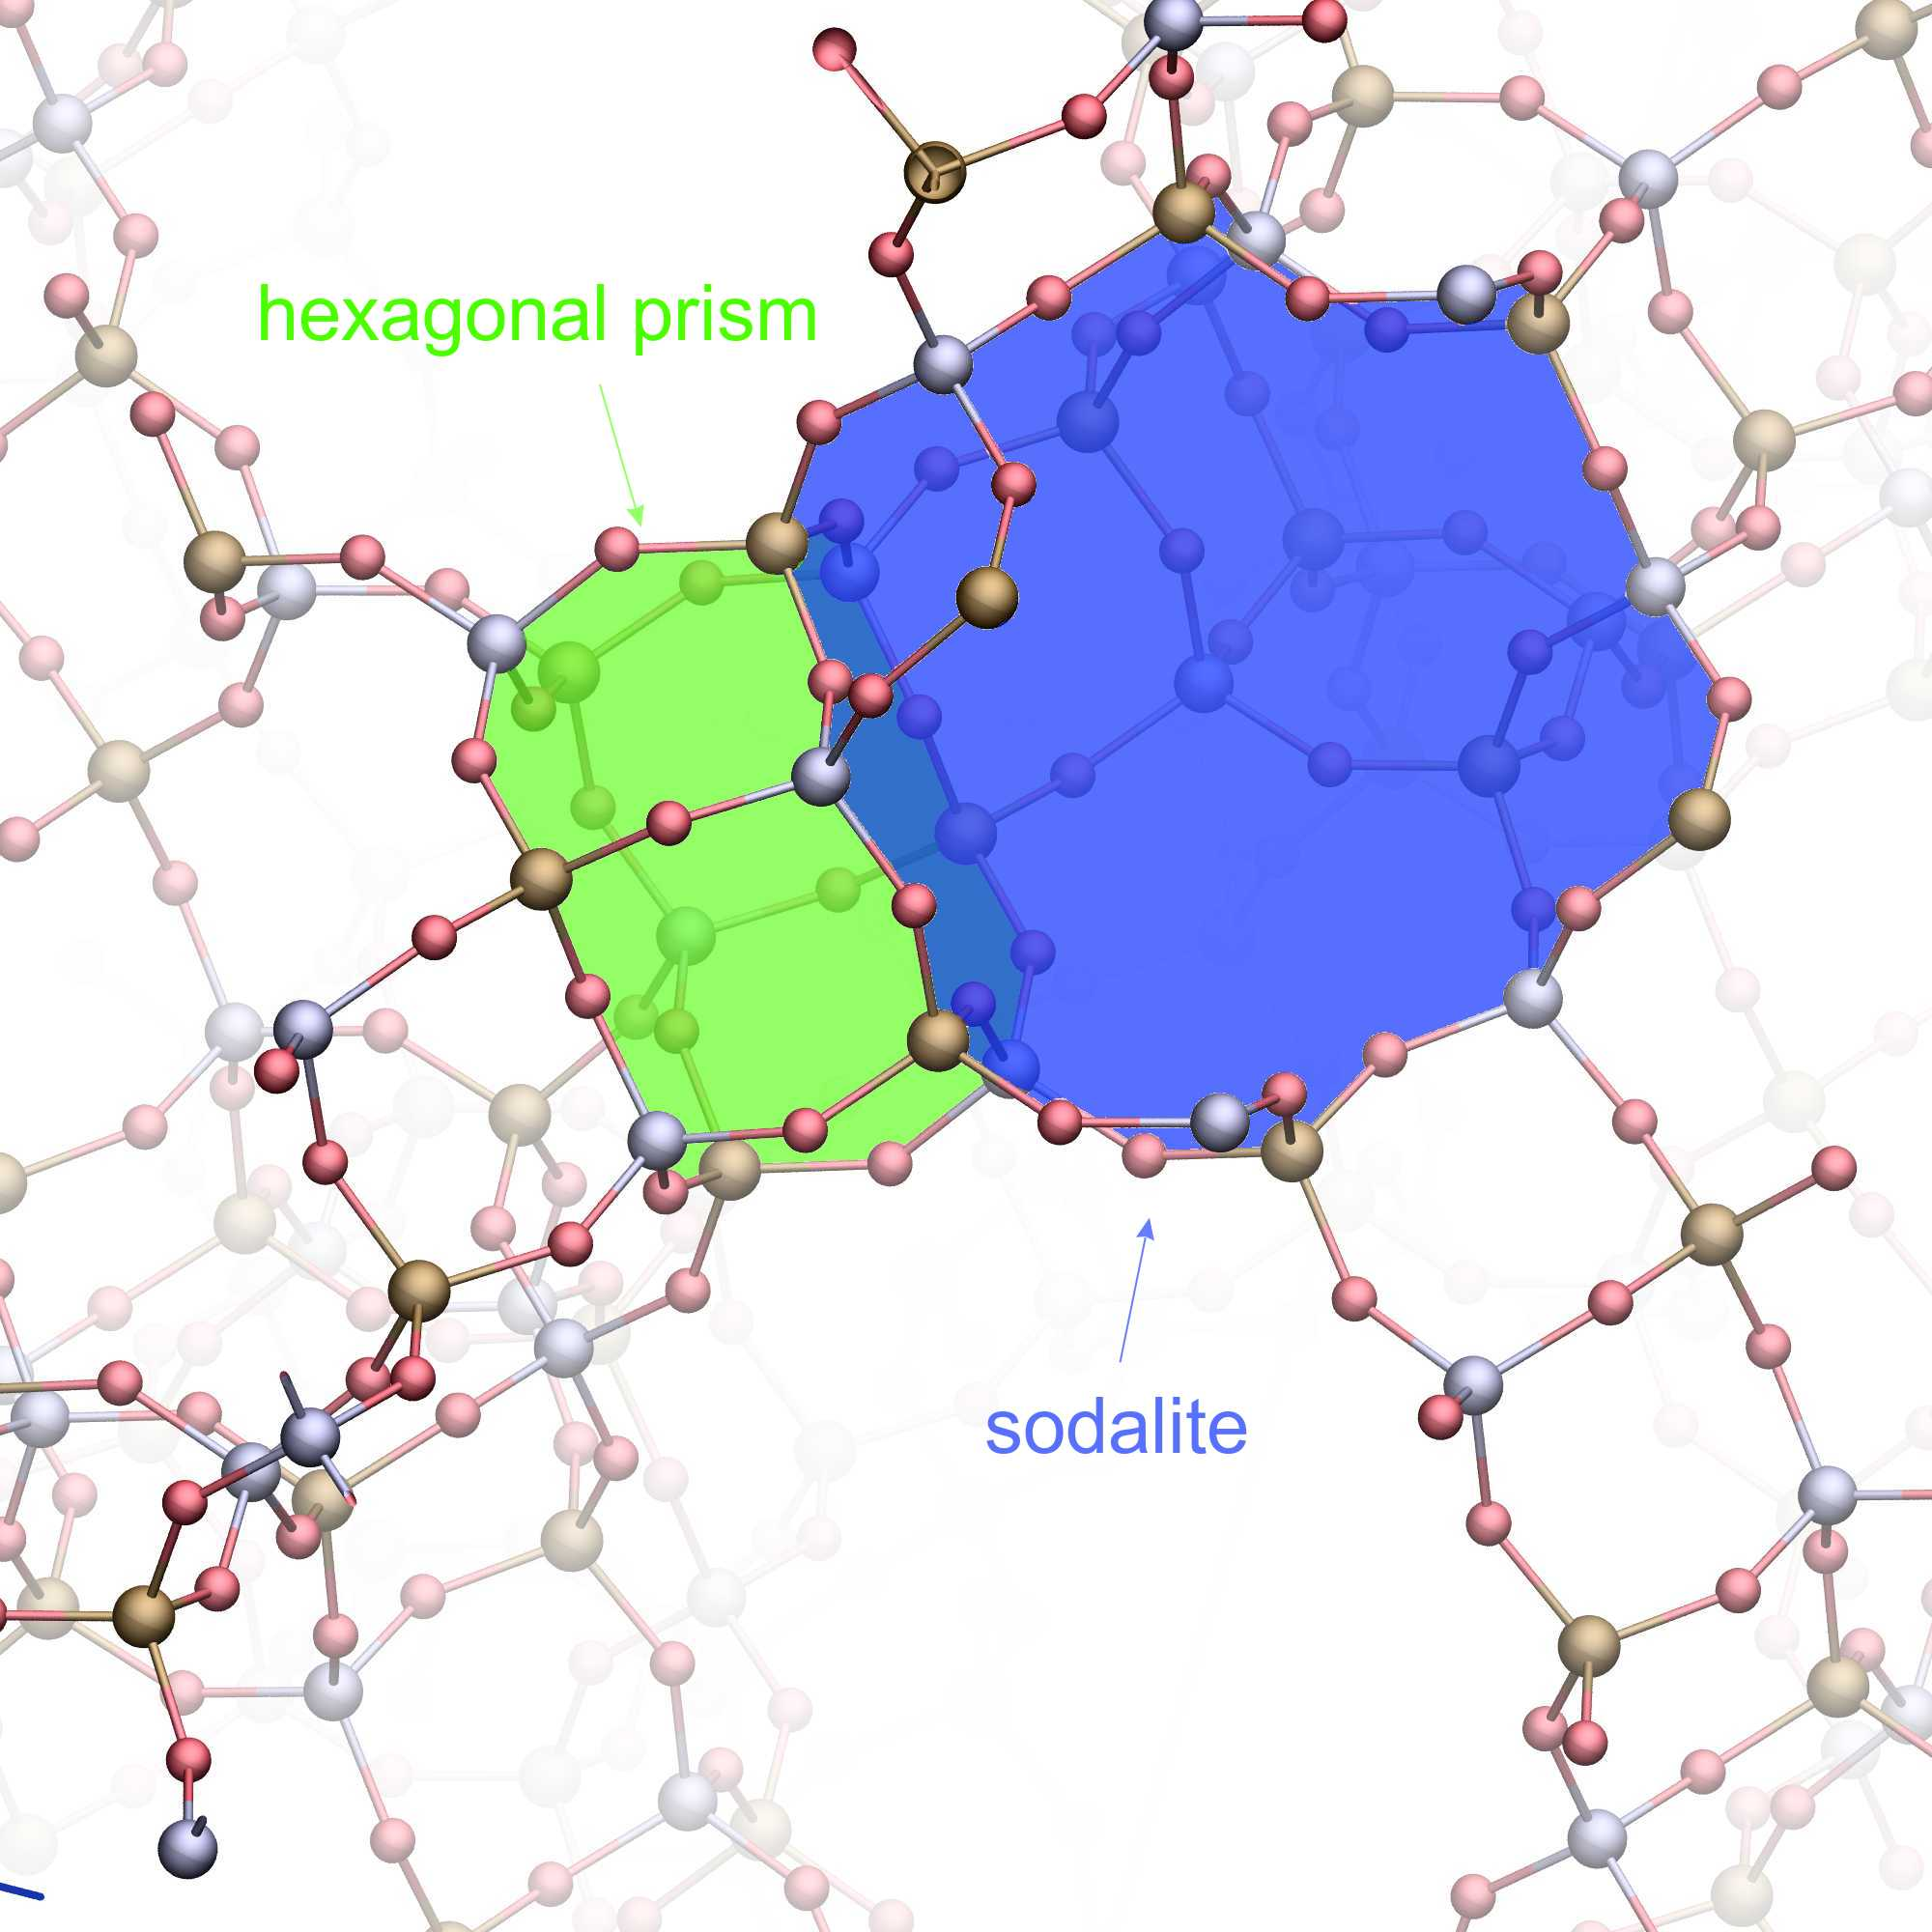
\includegraphics[width=0.95\columnwidth]{figures/cations/FAU1_cages_text.jpg}
		\subcaption{Détail des cages de la faujasite}
	\end{subfigure}\hfill%
	\begin{subfigure}{0.45\columnwidth}
		\centering
		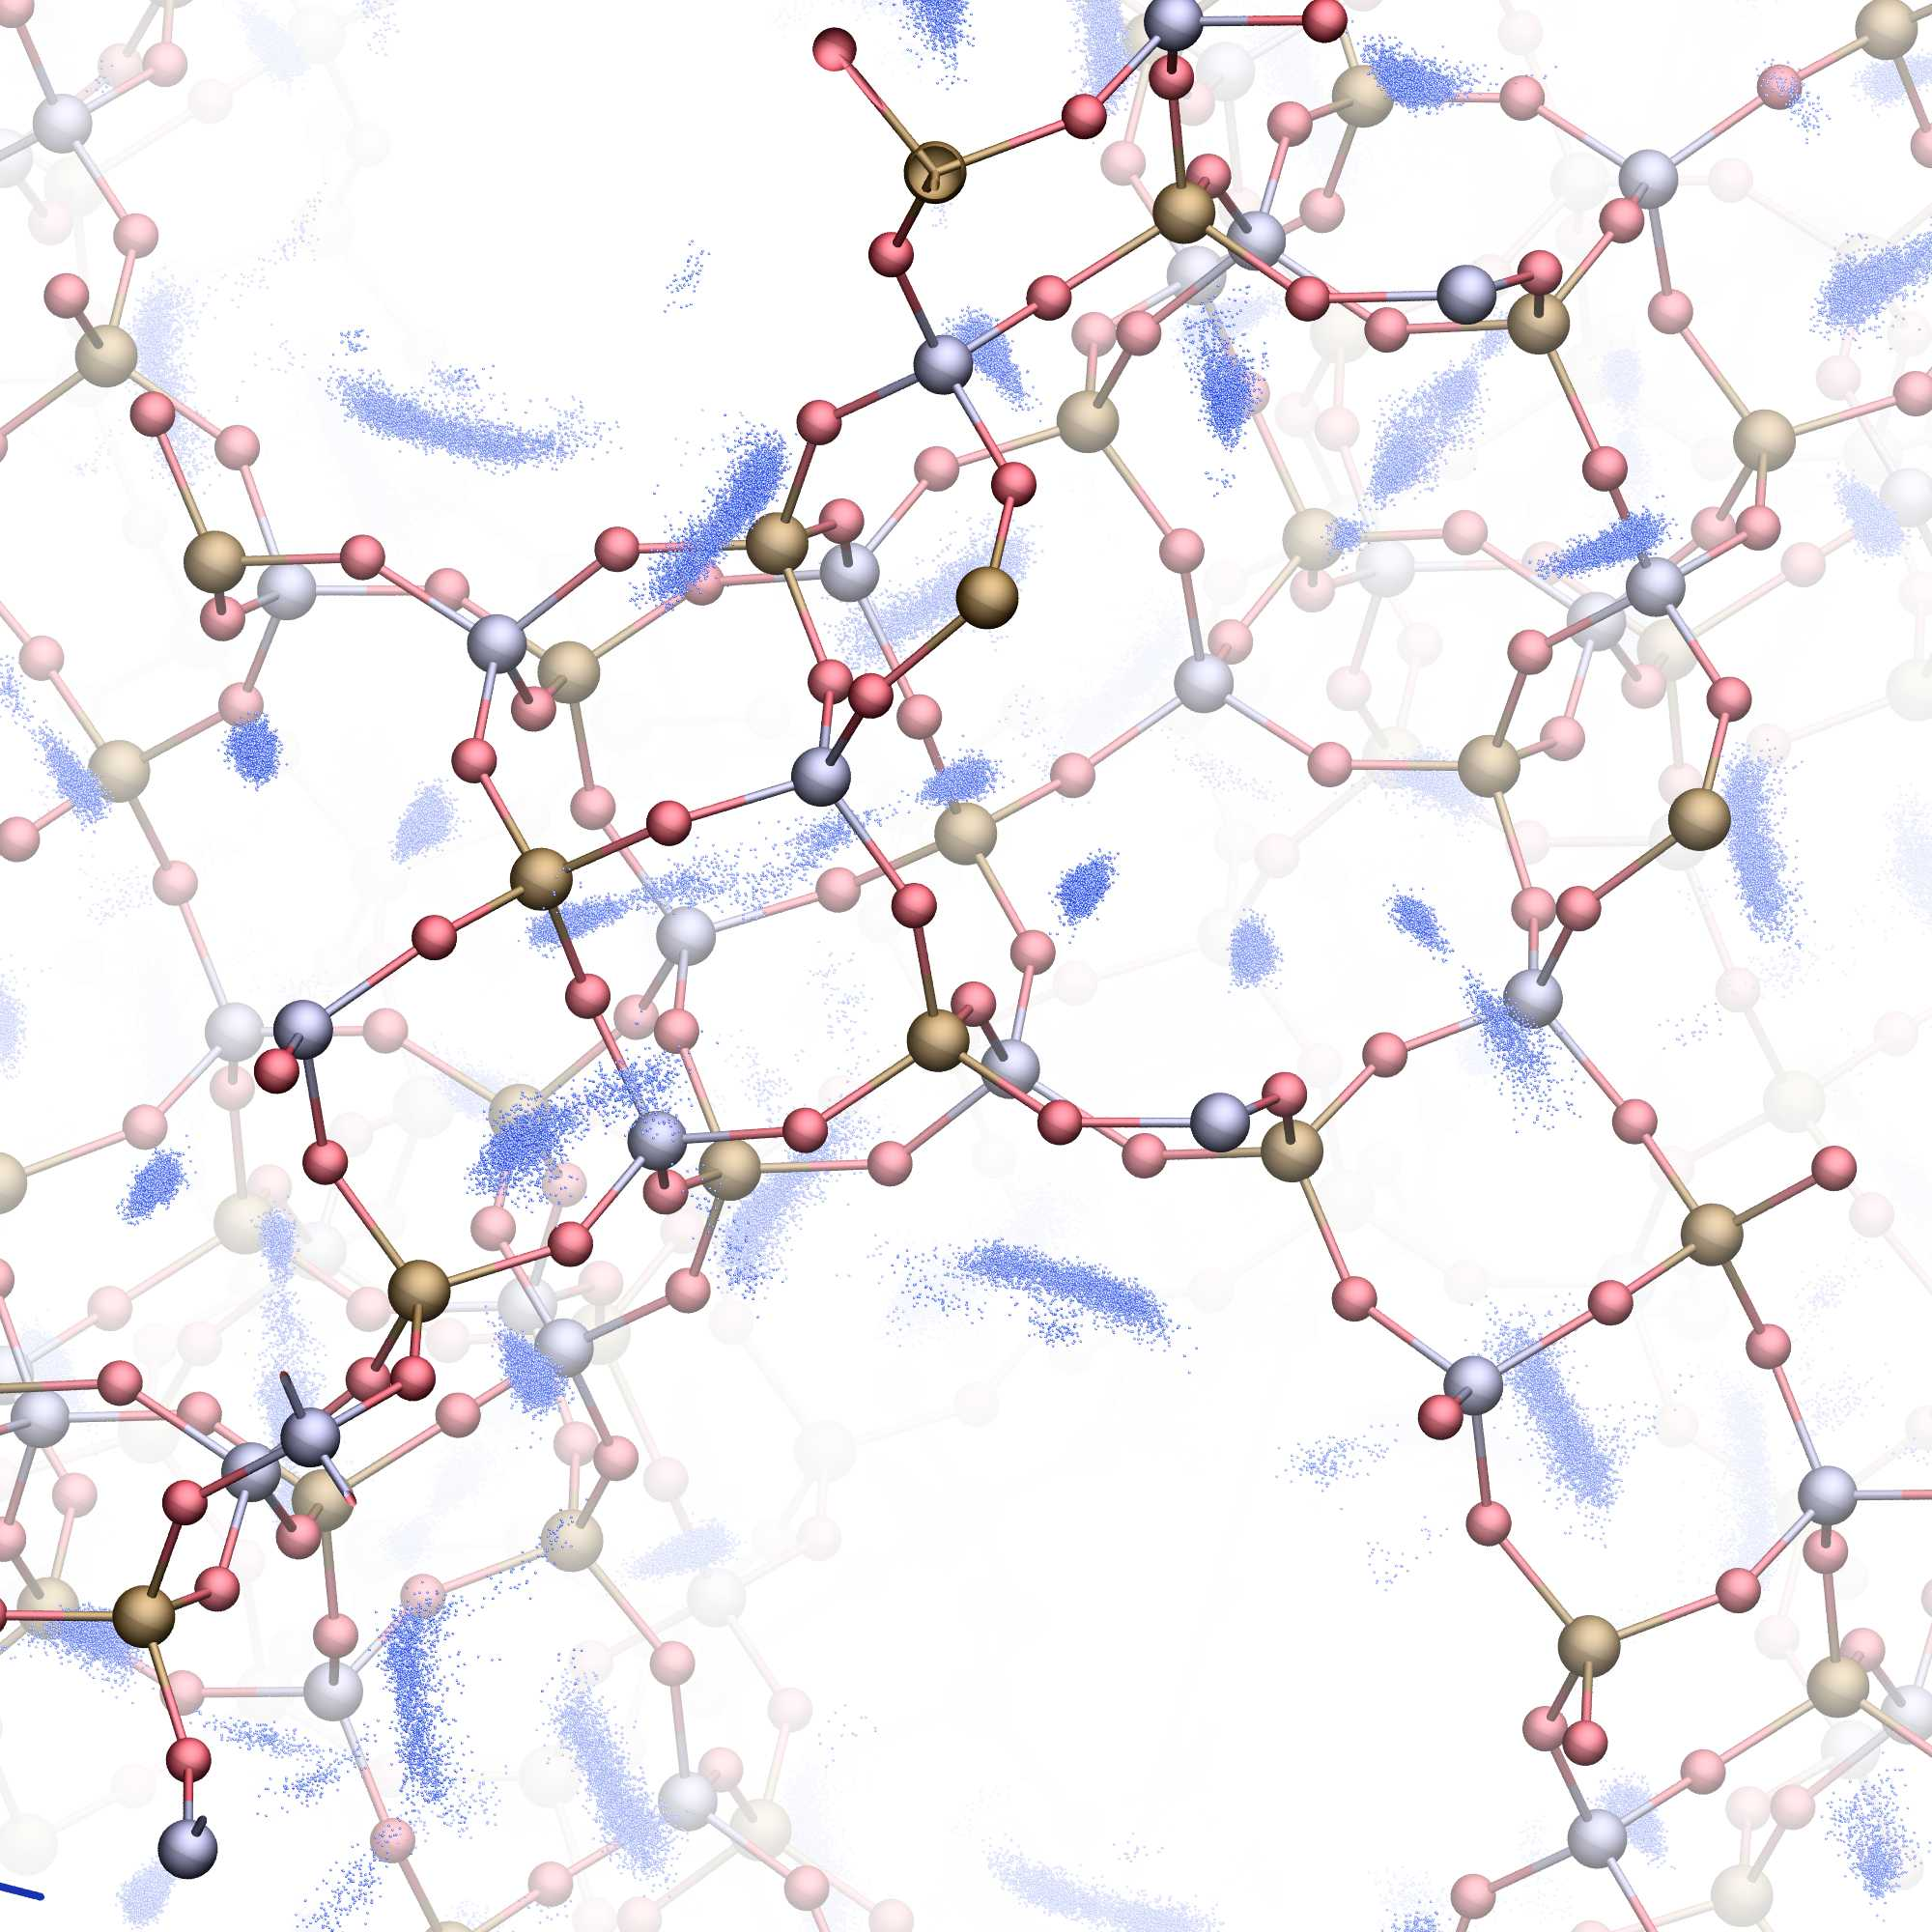
\includegraphics[width=0.95\columnwidth]{figures/cations/FAU1_density.jpg}
		\subcaption{Carte de densité cationique}
	\end{subfigure}\hfill
	
	\vspace{0.5em}
	
	\hfill\begin{subfigure}{0.45\columnwidth}
		\centering
		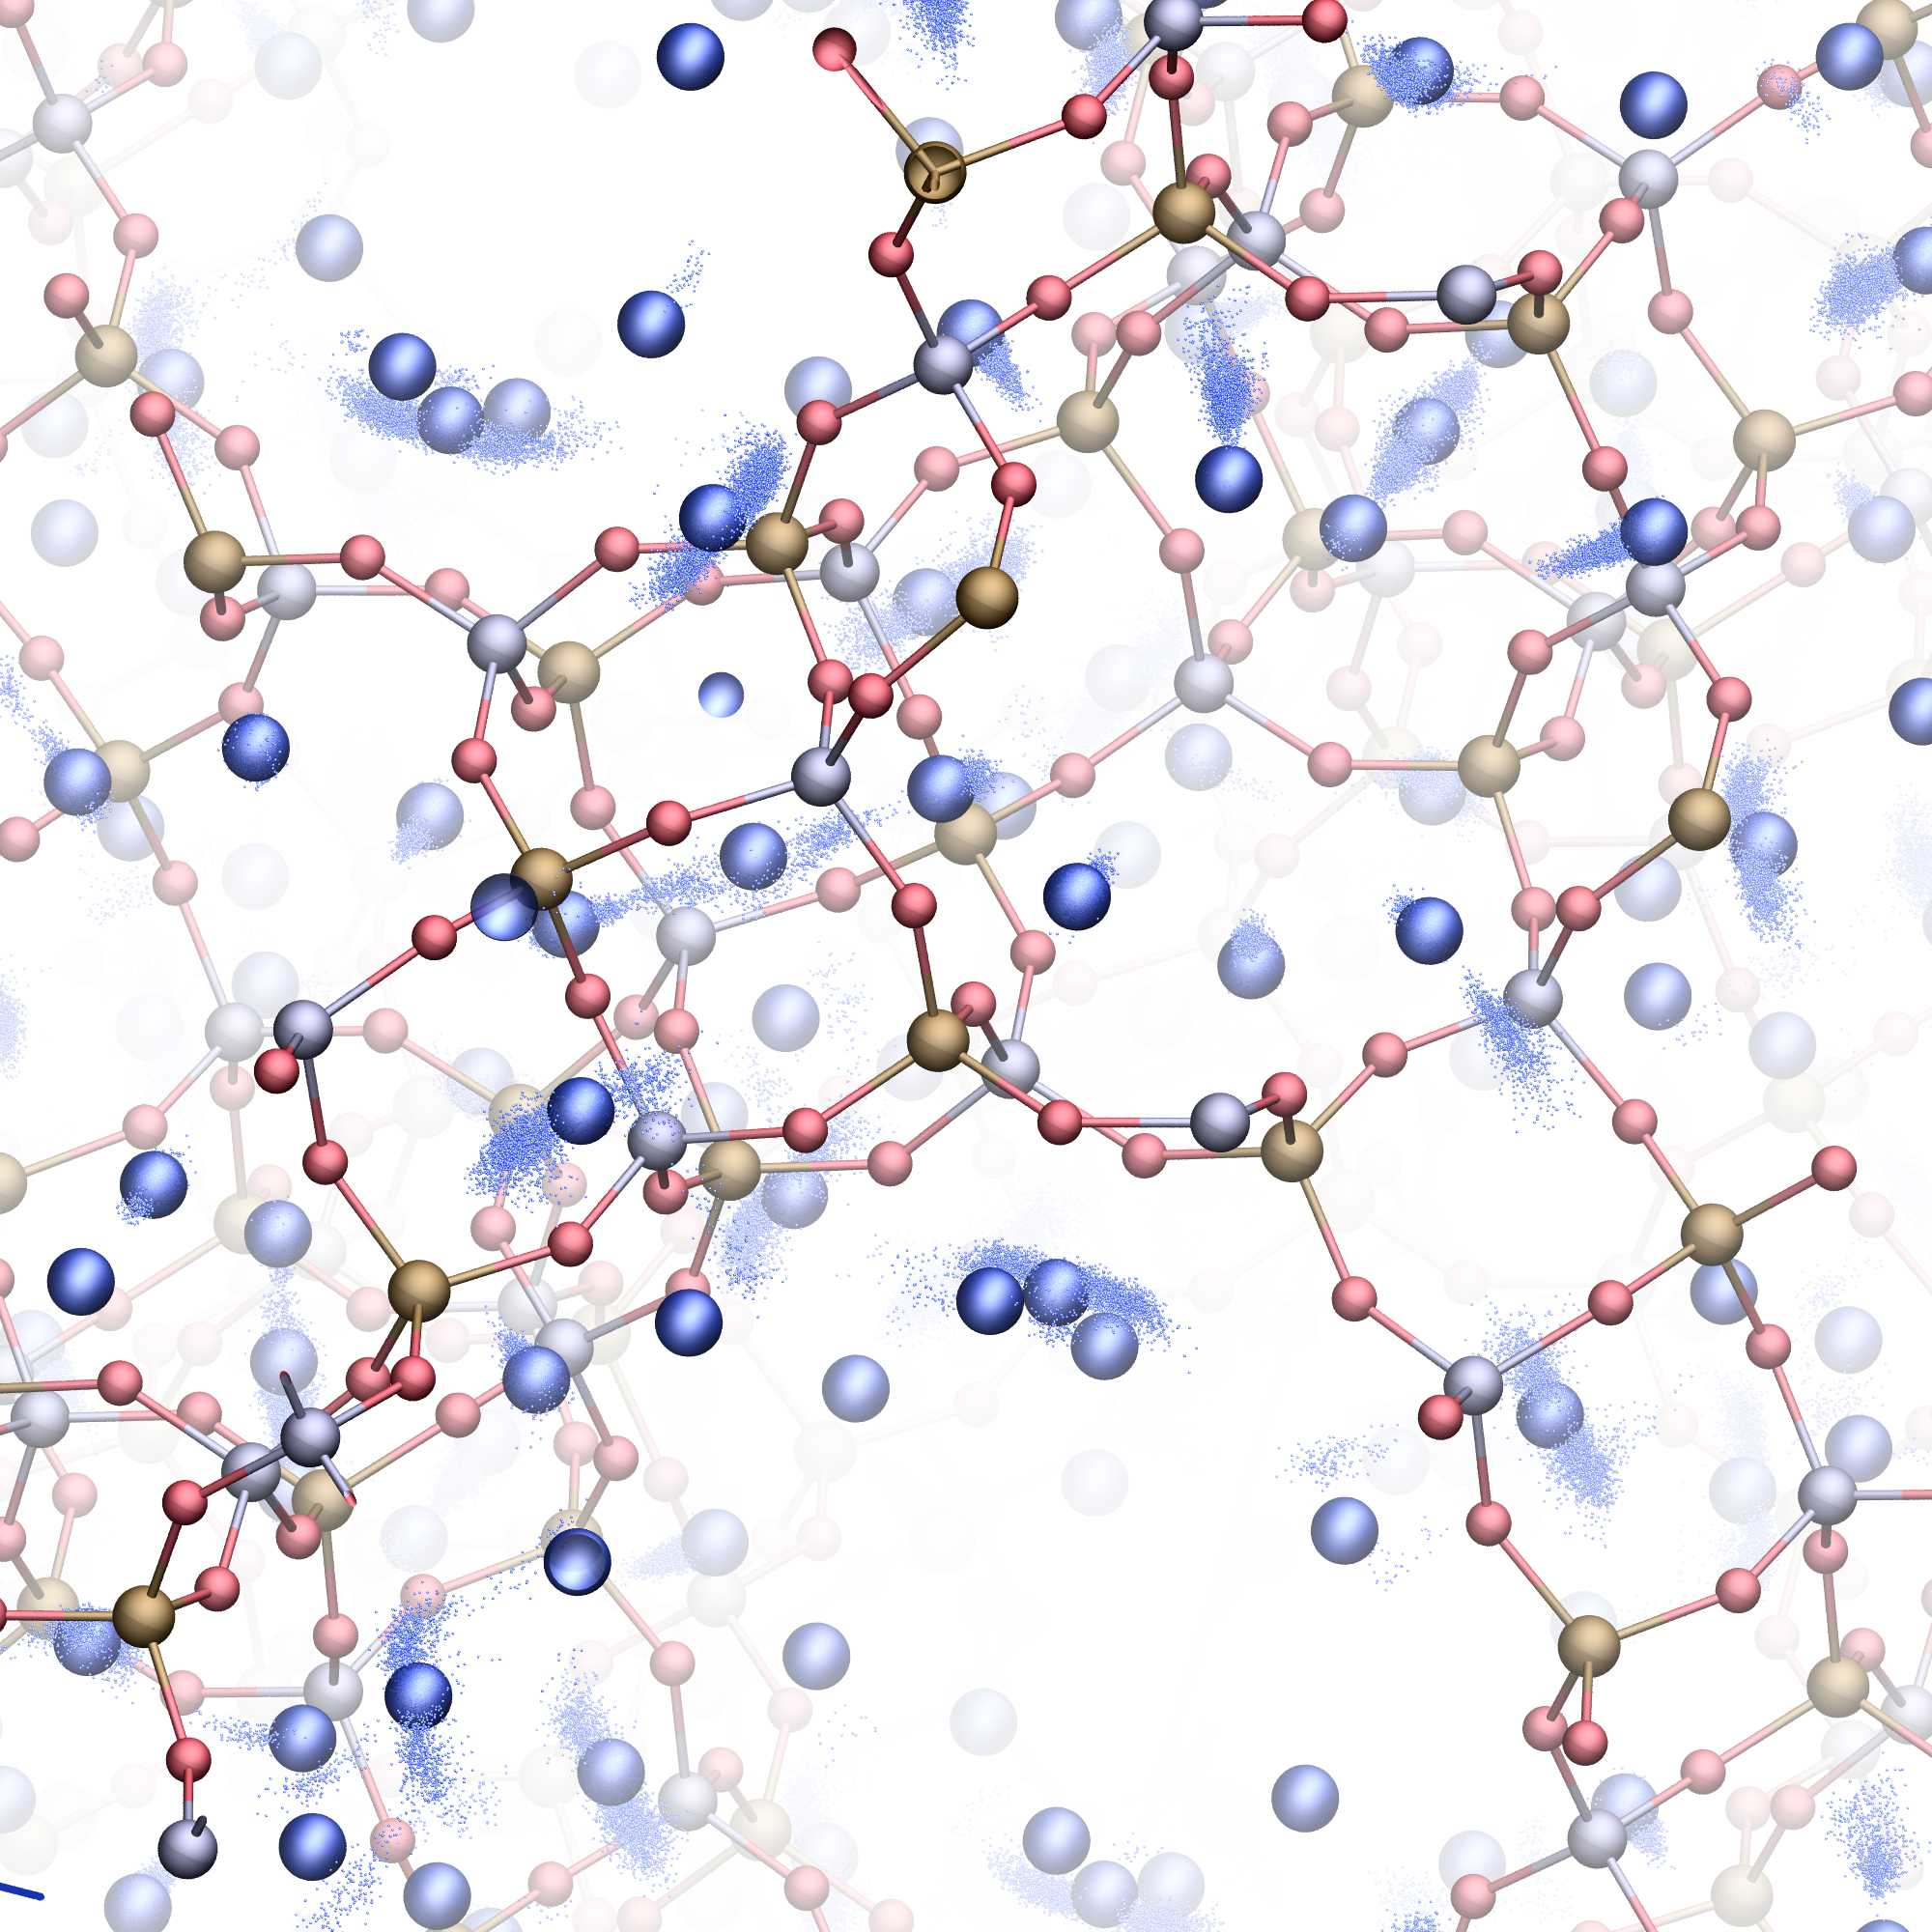
\includegraphics[width=0.95\columnwidth]{figures/cations/FAU1_density_Na.jpg}
		\subcaption{Extraction des sites depuis la carte de densité}
	\end{subfigure}\hfill%
	\begin{subfigure}{0.45\columnwidth}
		\centering
		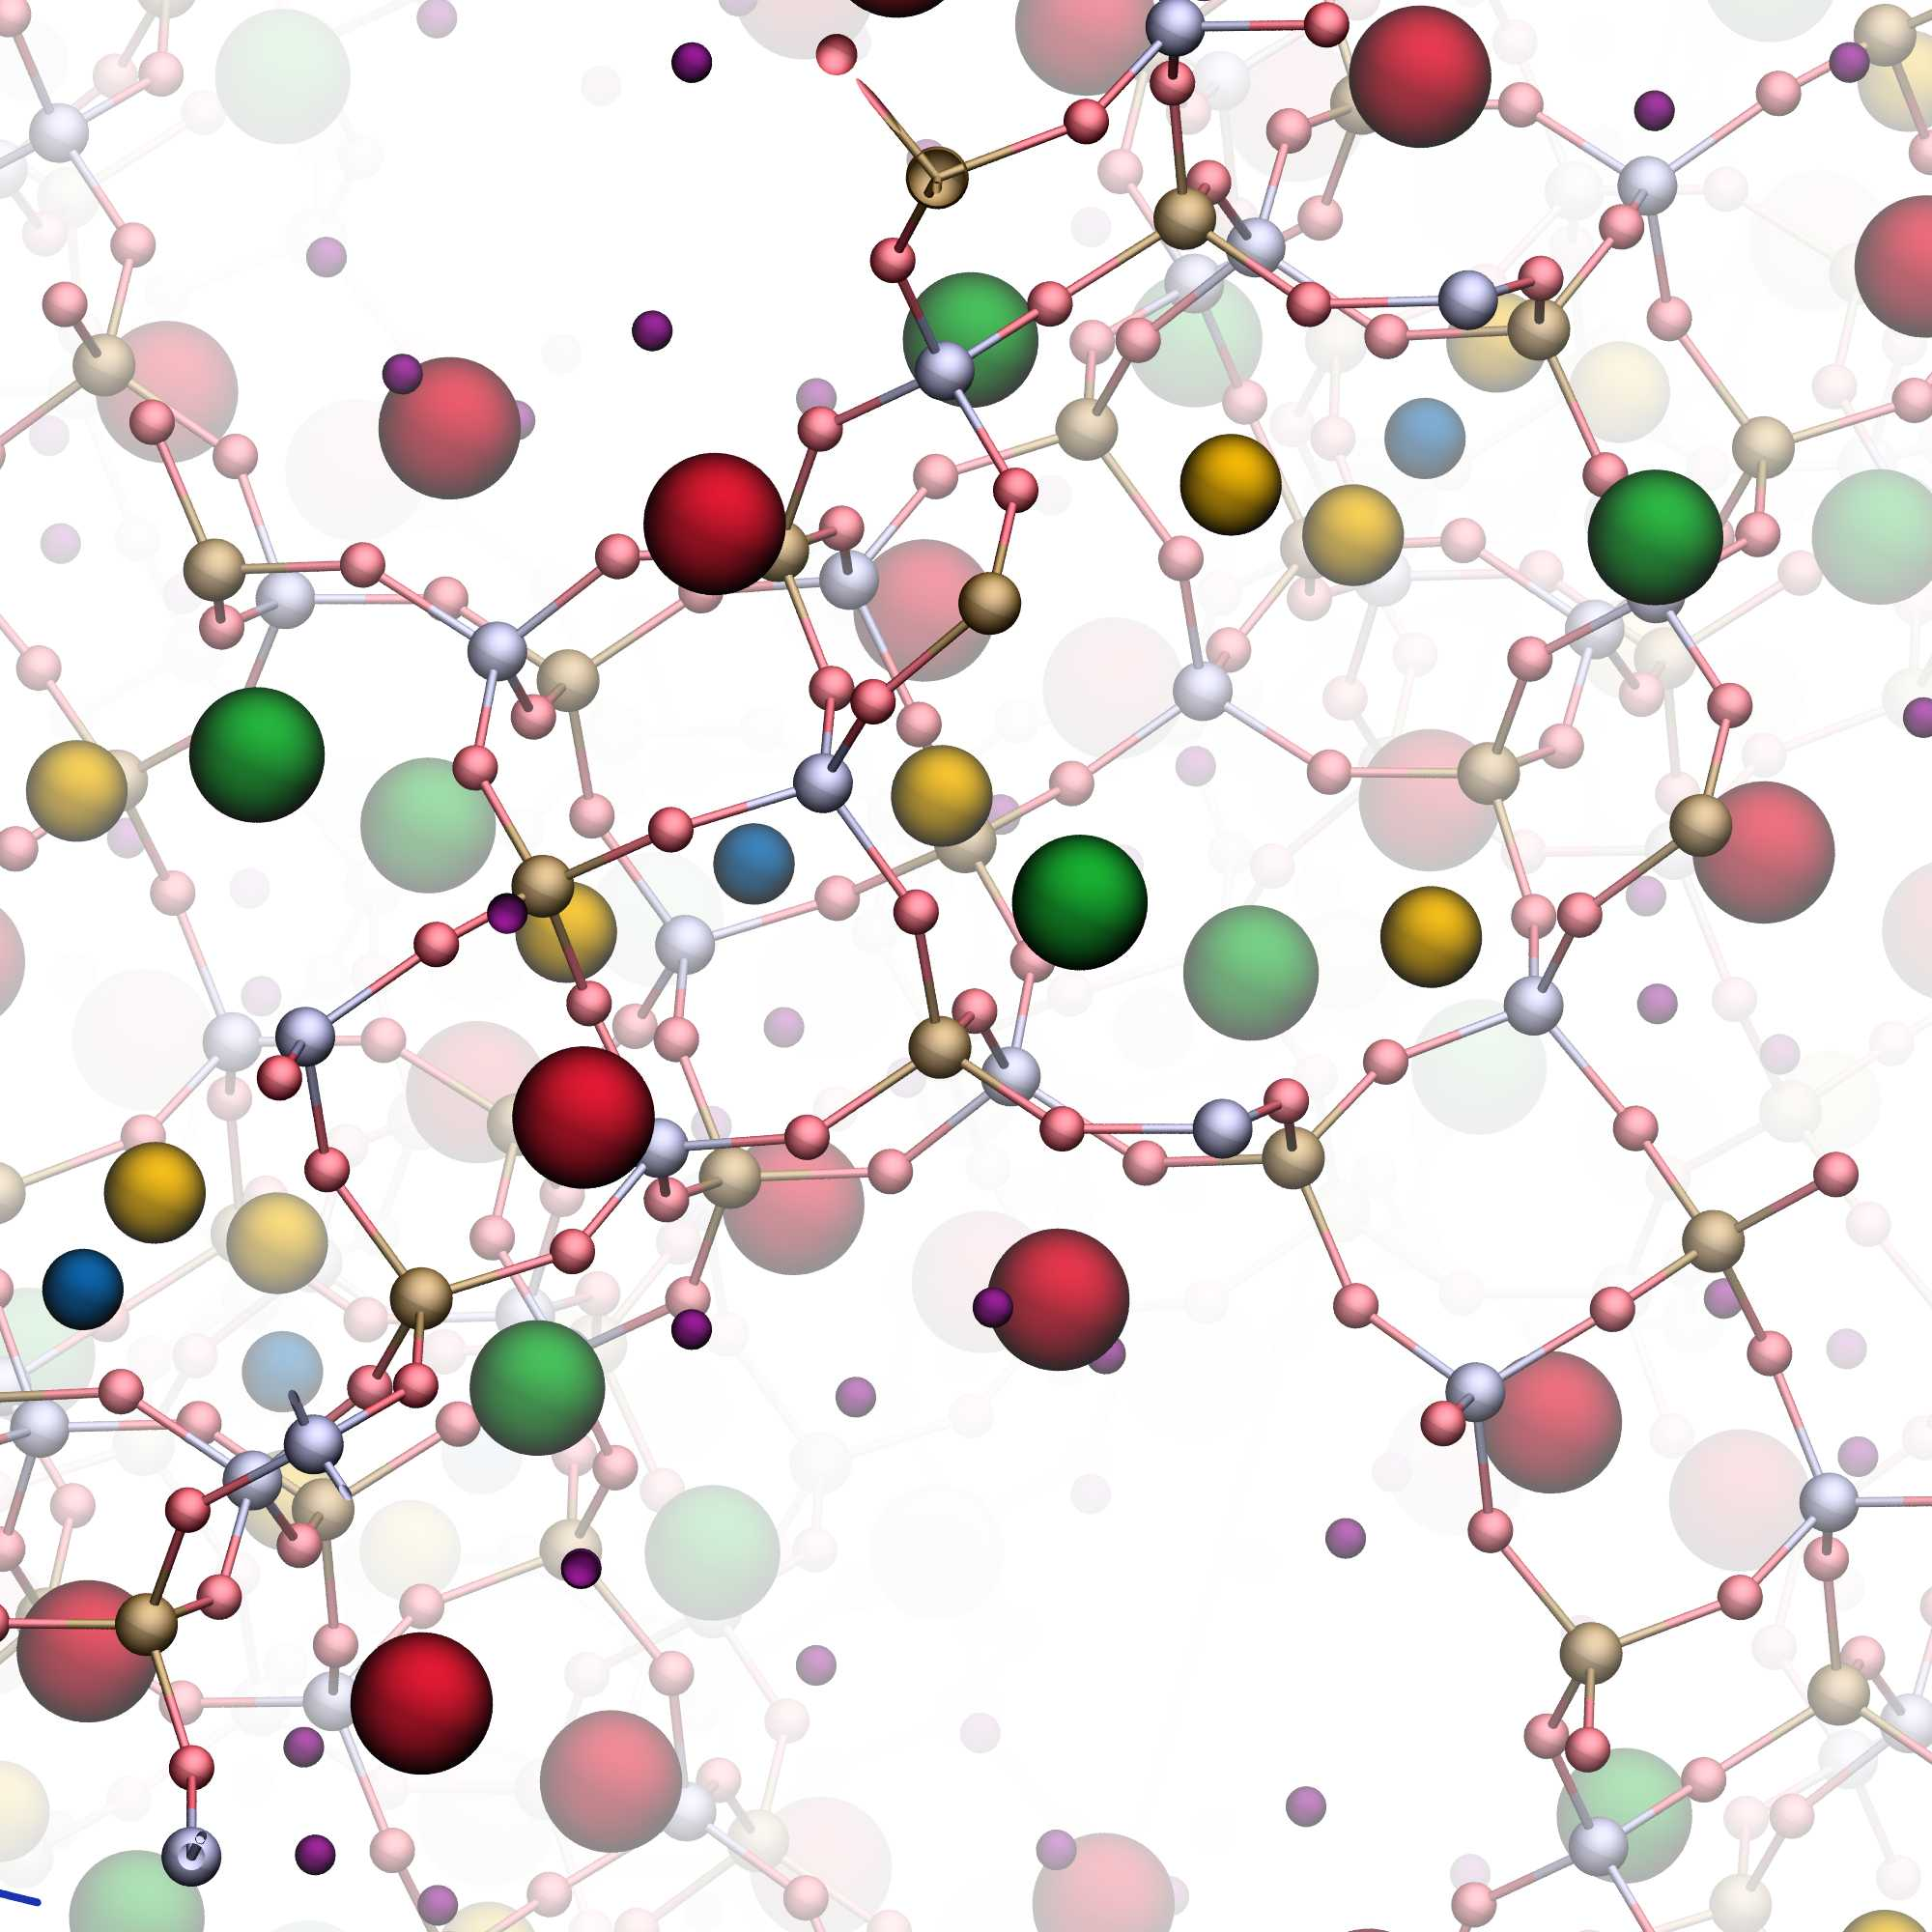
\includegraphics[width=0.95\columnwidth]{figures/cations/FAU1_NaColors.jpg}
		\subcaption{Sites cationiques après re-symétrisation}\label{fig_FAU_sites}
	\end{subfigure}\hfill
	
	\caption{Localisation des cations dans la faujasite. Les couleurs de la \cref{fig_FAU_sites} correspondent aux différents sites uniques ; leur taille est proportionnelle à leur occupation lorsque $\SiAl = 1$.}\label{fig_FAU}
\end{figure}

La dernière étape consiste à produire des modèles atomistiques de zéolites où chaque cation a une position unique, et non pas une probabilité de présence sur chaque site comme précédemment. Il suffit pour cela d'utiliser des instantanés issus des simulation de saut de site en site : pour chaque zéolite et rapport \SiAl étudié, pour chacun des 6 modèles où les aluminiums sont placés, j'ai gardé 6 placements distincts des cations.


\section{Simulation moléculaire de l'adsorption}

\subsection{Monte-Carlo grand canonique}

À l'échelle moléculaire, l'adsorption résulte d'interactions de van der Waals ainsi que coulombique, des atomes du matériau sur les atomes des espèces gazeuses. Tout comme pour le placement des cations, il est possible de simuler le comportement du gaz dans un modèle de zéolite, et même de prédire la capacité d'adsorption, c'est-à-dire le nombre moyen de molécules restant dans la zéolite en moyenne lorsqu'elle est mise en contact avec un réservoir de gaz à une température et une pression fixée.

Cette pression du gaz à l'extérieur se traduit par une valeur fixée du potentiel chimique du gaz à l'intérieur des pores du matériau. On utilise donc une simulation dans l'ensemble grand canonique : dans l'implémentation, cela requiert d'ajouter des pas Monte-Carlo d'insertion et de suppression des molécules, ce qui complexifie légèrement le code. Le logiciel open-source RASPA \autocite{RASPA} permet déjà d'effectuer de telles simulations ; j'ai réimplémenté les éléments nécessaires dans une version simplifiée pour jouir d'une meilleure performance.

\subsection{Monte-Carlo sur grille}

Afin d'obtenir des capacités d'adsorption en grand nombre, sur de très nombreuses zéolites, il est crucial d'utiliser une méthodologie optimisée. Dans cette optique, j'ai étudié une méthodologie simplifiée dans laquelle les molécules de gaz sont contraintes d'évoluer sur une grille tridimensionnelle, conceptuellement similaire aux simulations de saut de site en site pour les cations, mais avec un nombre bien plus important de sites puisqu'il y en a autant que de points de grille.

Cette approche donne de très bons résultats pour les molécules mono-atomiques : dans le cas de l'argon, le résultat est indistinguable de ceux obtenus par la méthode précédente. Pour les autres molécules cependant, la précision s'effondre dès que les interactions molécules-molécules cessent d'être négligeables, donc aux pressions supérieures à \qty{0.1}{MPa}. Ce résultat est indépendant de la taille de la grille choisie, ce qui souligne que cette limitation est intrinsèque à cette stratégie de simulation. Ces résultats sont représentés sur la \cref{fig_gridMC-ArMFI}.

\begin{figure}[ht]
	\centering
	\begin{subfigure}{0.48\linewidth}
		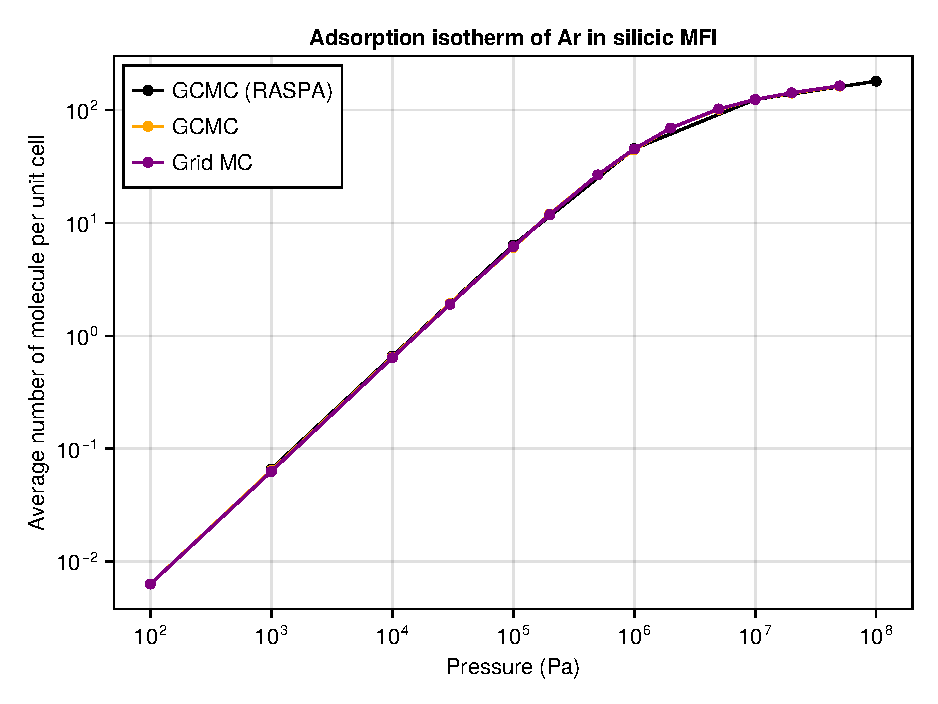
\includegraphics[width=\columnwidth]{figures/gcmc/gridmc_Ar_MFI.pdf}
		\subcaption{Reproduction parfaite de l'isotherme d'adsorption avec la méthode sur grille (ligne violette) comparée à la stratégie normale (en noir par RASPA, en orange par mon implémentation) pour la molécule mono-atomique d'argon sur la silicalite.}
	\end{subfigure}\hfill%
	\begin{subfigure}{0.48\linewidth}
		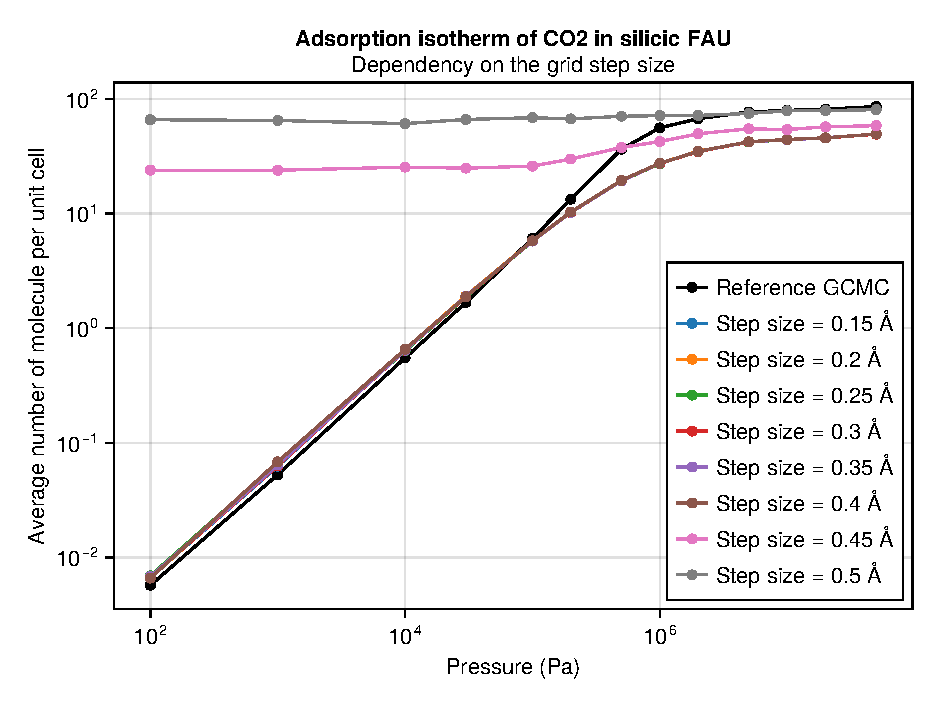
\includegraphics[width=\columnwidth]{figures/gcmc/gridmc_CO2_FAU_comparison_size.pdf}
		\subcaption{Déviations de l'isotherme d'adsorption avec la méthode sur grille quasiment indépendante du pas de la grille, comparée à la stratégie normale (en noir) pour la molécule poly-atomique de dioxyde de carbone sur la faujasite.}
	\end{subfigure}
	\caption{Comparaison du Monte-Carlo grand canonique et de la version sur grille pour des espèces mono-atomiques et poly-atomiques}\label{fig_gridMC-ArMFI}
\end{figure}


\section{Apprentissage statistique des isothermes d'adsorption}

La combinaison des deux sections précédentes permet d'obtenir, pour toute zéolite, un protocole de simulation permettant de prédire sa capacité d'adsorption pour n'importe quel gaz, pour tous choix de cation, rapport \SiAl, température et pression fixés. La précision du résultat est alors fonction de la qualité du calcul d'énergie choisi, à partir d'un champ de force classique ou de la théorie de la fonctionnelle de la densité par exemple.

Le temps de calcul de chacune de ces étapes reste cependant considérable, aussi il serait souhaitable de disposer d'un outil pour pouvoir prédire grossièrement mais très rapidement ces capacités d'adsorption, sans avoir à effectuer de simulation. Dans cette optique, j'ai commencé à créer une base de donnée de laquelle je propose quelques modèles statistiques simples pour prédire les isothermes d'adsorption.

\subsection{Isothermes d'adsorption}

Expérimentalement, une méthode assez commune de caractérisation de la porosité d'un matériau consiste à tracer son isotherme d'adsorption, c'est-à-dire l'évolution de sa capacité d'adsorption en fonction de la pression, pour une température et un gaz donnés. Ces courbes ont une forme particulière que l'on peut modéliser grâce à des modèles d'isothermes connus dans la littérature, comme celui de Langmuir, entre autres \autocite{AyaweiIsothermModels}.

\subsection{Modèle statistique}

Une fois un modèle d'isotherme choisi, les propriétés d'adsorption d'une zéolite se résument à l'évolution des différents paramètres du modèle en fonction de la température, du rapport \SiAl, du gaz et de la nature du cation. En fixant le gaz, soit à \ce{CO2} soit à \ce{N2}, et le cation à \ce{Na+}, j'ai construit quelques méta-modèles simples qui donnent l'évolution des paramètre d'un modèle d'isotherme en fonction de la température et du rapport \SiAl pour trois topologies de zéolites (FAU, LTA et CHA).

\begin{figure}[b]
	\begin{subfigure}{0.49\columnwidth}
		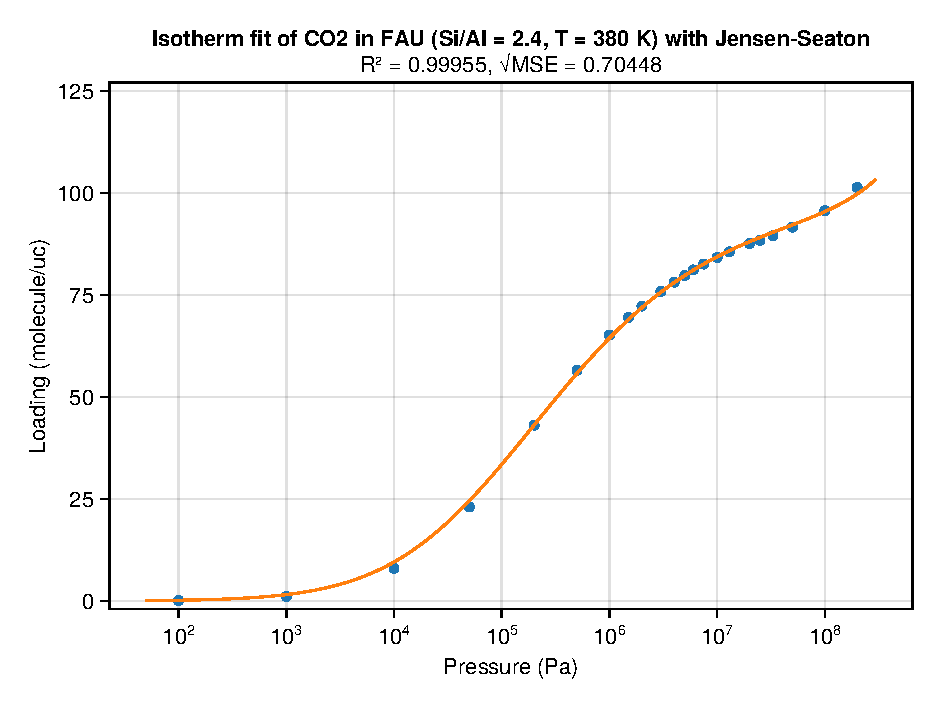
\includegraphics[width=\columnwidth]{figures/isotherms/referencefit_jsfit.pdf}
		\subcaption{Fit avec le modèle d'adsorption de Jensen-Seaton}
	\end{subfigure}\hfill%
	\begin{subfigure}{0.49\columnwidth}
		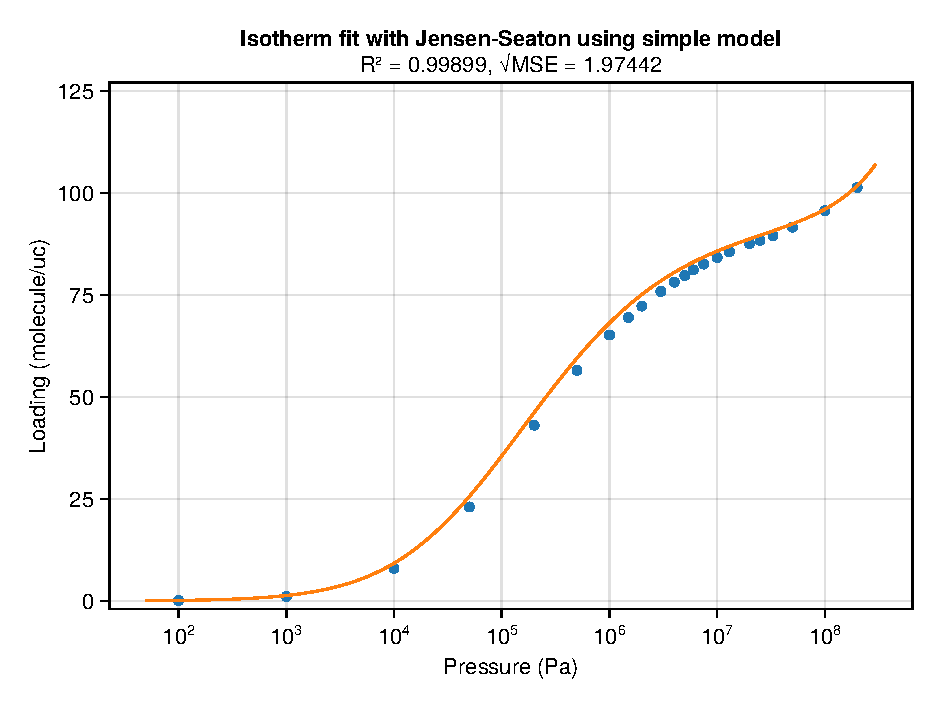
\includegraphics[width=\columnwidth]{figures/isotherms/referencefit_simplemodel.pdf}
		\subcaption{Isotherme obtenue avec le méta-modèle}
	\end{subfigure}
	\caption{Isothermes d'adsorption du \ce{CO_2} dans la faujasite avec $\SiAl = 2.4$ à \qty{380}K}\label{fig_simplemodelfit}
\end{figure}

Un exemple est donné sur la \cref{fig_simplemodelfit}, où l'isotherme retrouvée grâce au méta-modèle est très semblable à celle obtenue directement en calant le modèle d'isotherme pris sur les données. Ces résultats préliminaires sont prometteurs, mais la base de donnée est encore en cours de construction au moment de l'écriture de cette thèse.

\section*{Conclusion}

Les matériaux cristallins nanoporeux forment la source principale d'adsorbants en usage pour les procédés industriels de séparation gazeuse. Pour trouver les candidats les plus prometteurs, des simulations numériques permettent de prédire leurs propriétés ; elles requièrent cependant une description du matériau. À l'échelle la plus fine, celle-ci nécessite la position de tous les atomes de la structure, pour pouvoir évaluer chaque interaction de paire ; au contraire, la seule topologie d'un matériau donne une idée très simplifiée de sa structure.

\texttt{CrystalNets.jl} est un nouvel outil que j'ai développé pour rendre cette notion de topologie plus accessible à la communauté scientifique, au travers de son interface web intuitive en particulier. J'ai aussi rassemblé d'autres outils d'analyse topologique, notamment de statistique d'anneaux, dans une autre bibliothèque, \texttt{PeriodicGraphs.jl}, lui aussi écrit en Julia.

Au sein des différentes familles de matériaux poreux, les zéolites cationiques sont parmi les plus utilisées dans l'industrie, mais la description atomistique de leur structure pose des problèmes particuliers. En effet, le placement de leurs aluminiums est difficilement mesurable expérimentalement, et la localisation de leurs sites cationiques est inconnue pour la majorité des topologies. J'ai proposé une méthodologie en plusieurs étapes pour retrouver des structures atomistiques plausibles, en partant d'un algorithme de marche aléatoire pour placer des aluminiums, puis en utilisant un nouveau méta-algorithme ``étoile filante'' pour obtenir les sites, ceux-ci étant ensuite utilisés dans une simulation de saut de site en site combinée avec un recuit simulé pour obtenir leur peuplement.

Une fois obtenue les positions de tous les atomes d'un matériau donné, la méthode de simulation Monte-Carlo grand canonique permet de retrouver la capacité d'adsorption du matériau. J'ai comparé cette méthode avec une stratégie simplifiée où les espèces mobiles sont contraintes à se localiser sur une grille : les résultats sont probants pour les molécules mono-atomiques, mais ne sont convenables pour les autres qu'aux basses pressions.

Une autre approche, statistique plutôt qu'atomistique, permet d'obtenir très rapidement des isothermes d'adsorption au moyen d'interpolations. Pour ce faire, j'ai commencé à constituer une base de données de telles isothermes pour \ce{CO2} et \ce{N2} dans les zéolites cationiques, pour différents rapports \SiAl, températures et pressions. La qualité du résultat est satisfaisant, mais la petite taille de la base de donnée ne permet pas encore de généraliser la prédiction des capacités d'adsorption à de matériaux non simulés.\\

Ce travail peut naturellement être étendus dans différentes directions. Un paramètre à étudier est sans doute la nature du cation, pour le moment cantonné à \ce{Na+}. Pour des fins de séparation gazeuse, une méthodologie spécifiquement dédiée à la coadsorption pourrait être pertinente. L'effet de l'eau mérite une attention particulière, car c'est un poison connu pour zéolites, dont l'hydrophilie augmente avec le nombre de cations. Enfin, l'adsorption de gaz peut avoir un effet sur le placement des cations dans les zéolites ; quantifier cette rétroaction est donc indispensable pour s'assurer de la qualité des mesures numériques de capacités d'adsorption.

Avant ces généralisations cependant, la prochaine étape de ce projet consiste à étendre la base de données d'isothermes d'adsorption avec plus de topologies. Ceci permettrait en effet de construire un modèle beaucoup plus général, pouvant intégrer la topologie du matériau dans ses paramètres d'entrée. À cette fin, il faudra cependant trouver des descripteurs topologiques pertinents, comme ceux dérivés du pavage topologique : ceci consiste en une décomposition de l'espace en volumes poreux séparés par des anneaux du réseau des liaisons chimiques du matériau. Ce pavage permet donc une analyse fine de la topologie des pores du matériau, en lien direct avec ses capacités d'adsorption, et sans doute avec la localisation des sites cationiques. Tout modèle prédictif requerra par ailleurs des descripteurs géométriques de la structure à étudier.

Atteindre un tel modèle permettrait théoriquement d'obtenir des isothermes d'adsorption réalistes et quasiment instantanées, pour toute combinaison de topologie zéolitique, rapport \SiAl et température. La précision du résultat pourrait même être dérivées des incertitudes sur les résultats des simulation sous-jacentes au modèle. À terme, ceci rendrait possible le criblage à ultra-haut débit des zéolites pour leurs capacités d'adsorption.

% \begin{figure}[h]
% \begin{minipage}[t]{.43\textwidth}
% \centering
%   \includegraphics[width=\linewidth]{figures/2-thermo/Enthalpy_0_log.jpg}
%   \caption{\small{\ Pour 8\,401 MOFs avec une sélectivité Xe/Kr favorable ($s\e{0} > 1$), pair-plots entre les différentes grandeurs $\log(s\e{0})$, $\Delta\e{exc}H\e{0}$, $\Delta\e{ads}H\ex{Xe}\e{0}$ et $\Delta\e{ads}H\ex{Kr}\e{0}$ (les enthalpies sont en \si{\kilo\joule\per\mol}) en dehors de la diagonale et la distribution de chaque grandeur sur la diagonale.}}\label{fgr:histo_H_resume}
% \end{minipage}
% \hfill
% \begin{minipage}[t]{.5\textwidth}
% \centering
%   \includegraphics[width=\linewidth]{figures/2-thermo/s_0_vs_s_2080_overview_log.jpg}
%   \caption{\small{\ Sélectivité à 1\,atm de pression en fonction de la sélectivité à basse pression pour une composition 20\pp{}80 Xe/Kr. Les points sont étiquetés selon la différence relative entre les deux sélectivités. Les points violets ont une grande différence relative entre les sélectivités. }}
%   \label{fgr:overview_resume}
% \end{minipage}
% \end{figure}


% \clearpage
% \section*{Conclusion}

% Texte \autocite{citation}

% \vfill
% \begin{center}
%     \pgfornament[width=6cm,color=CTsemi]{75}
% \end{center}
% \vfill\vfill

\end{otherlanguage}

\OnlyInSubfile{\printglobalbibliography}

\end{document}
